% Use the temporary template.
\documentclass{aer1315-pretty}

\usepackage{hyperref}
\usepackage{amsmath,amssymb}
\usepackage{eulervm}  % make math text non-italicized

% Author information
\author[]{ %
Christopher Ngigi\thanks{Graduate Research Assistant, Student ID: 999048230}\\
\textit{Institute for Aerospace Studies, University of Toronto}}

% Title
\title{Continuous Descent Approach: Benefits and Challenges}

% Abstract
 \abstract{ %
  This Interim Report investigates the effectiveness of Continuous Descent Approaches (CDA) which are part of Tailored Approaches (TA). Literature review of reports and publications indicating benefits of these are critiqued, and applicability as a whole analyzed. Findings from these sources are summarized.}


% Begin the document
\begin{document}
% Insert the title.
\maketitle

%%=======================================================================================================================
\section{Introduction}
While the aviation sector strives to reduce fuel consumption primarily for financial reasons, there is a growing awareness of its impact on the environment. We are still many years away from  resources being fully committed to the manufacture of breakthrough radical designs such as Blended Wing Bodies (BWB) which would significantly reduce the environmental footprint. These challenges stem from the expensive transition to new design procedures, since there is already a long-established and efficient interconnectivity that has been established by the major manufacturers with their subcontractors. Changes would potentially meet with certain resistance considering the high capital costs e.g. manufacturing equipment would need to be changed and replaced by an initially expensive process. Some of the newest entrants are utilizing new techniques to construct sections of aircraft fuselage such as the wings, tail sections and wing-box structures (i.e. the Boeing 787, Airbus A350, and Airbus A380). However, since these are still of conventional tube-and-wing configurations,  it is safe to say that it will be a long while  before any radical designs come into the market, and when they do, there may be the challenge of social acceptance.\par

Until this time arrives, we can try to improve the \textit{current} handling and operation of aircraft. We need to find techniques to alleviate the surging rise in fuel emissions, (particularly $CO_2$ - which has a potential life cycle of 200 years) due to the increasing popularity and need for air travel. How can we lower fuel consumption? Manufacturers have now began in earnest to use composite materials for some sections of aircraft fuselages, as mentioned above. Weight reductions have already been implemented by airline management to streamline efforts to reduce fuel consumption (financial motivation) - such as limiting the weight of checked luggage. Some airlines are implementing usage of Electronic Flight Bags (EFBs) in the cockpit as a weight-savings replacement to paper charts - Lufthansa even boasts of this on their website \cite{Lufty}. In terms of new materials and weight reduction, there is a current boom.\par




\begin{figure}[!h]%{wrapfigure}[31]{l}{0.5\textwidth}
  %\centering
   \subfigure[The Aviation Sector is responsible for approximately 5\% of emissions produced by the Transportation sector]
   {\label{fig:Emissions}	   
   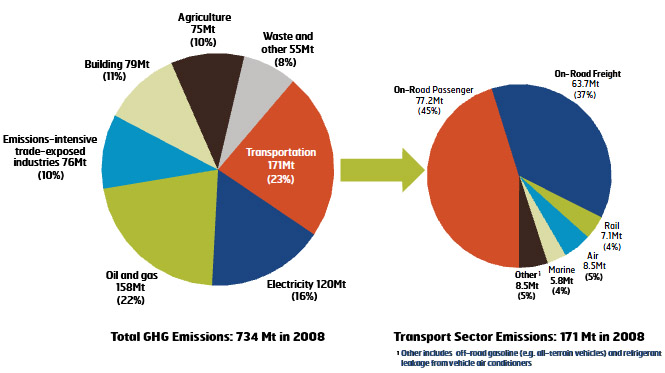
\includegraphics[height=0.28\textwidth, trim=0.2cm 0.2cm 0.2cm .2cm,clip=true]{figures/reduce_gas_emissions2.jpg}}
	\:
	\subfigure[Historical and projected reductions in $CO_2$ Emissions as provided by Transport Canada]
   {\label{fig:CO2}	   
   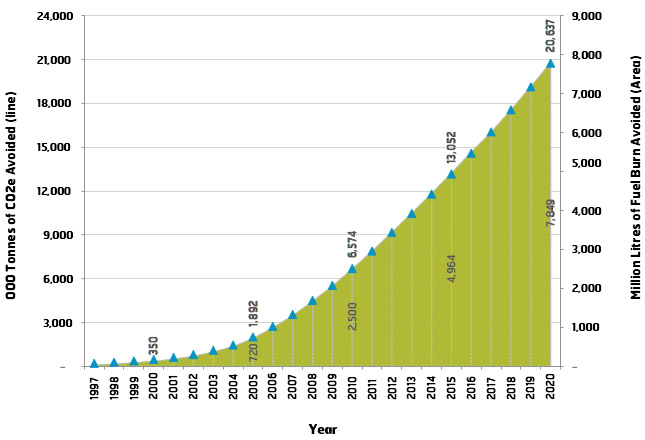
\includegraphics[width=0.45\textwidth, trim=0.2cm 0.2cm 0.2cm .2cm,clip=true]{figures/reduce_gas_emissions.jpg}}%
    \caption{Emissions from aviation data provided by Transport Canada \cite{TransportCanada}}  
\end{figure}

%%--------------------------------------------------------------------------------------------
\subsection{Pollution}

Presently, there is heavy emphasis on the control of pollution from the aviation sector, since it is a fast growing industry, projected to grow at an annual rate of 3-4\%. Data provided by Transport Canada \cite{TransportCanada} in \ref{fig:Emissions} shows that aviation is responsible for approximately 5\% of the entire transportation sector emissions (approximately 1\% of total greenhouse emissions).\par  

Engine manufacturers are continuously improving and refining engine design. An interesting observation is that there is current emphasis on reduction of $NO_x$ emissions. Within the engine, $NO_x$ formation occurs via the Zeldovich mechanism primarily in diffusion (non-premixed) type combustors. Diffusion type flames have a high primary zone temperature, which increases the production of thermal $NO_x$. The trend now is to implement partial-premixing, (i.e. mixing of air with fuel prior to entry into the combustion chamber, reducing the primary zone temperature, and consequently $NO_x$. However, the adverse effect is an increase $CO_2$ and Unburned Hydro Carbons (UHCs) emission. It is difficult to pit a pollutant against another, but based on time effects, $NO_x$ has a projected lifespan of approximately 2 weeks, while $CO_2$ nearly 200 years. $CO_2$ is a greenhouse gas that effectively raises the Earth's average temperature, and rather unfortunately, takes a very long time before it is re-absorbed.\par

Other pollutants such as $NO_x$, Aircraft Induced Cirrus are also harmful, however, $CO_2$ will be considered a principal target for emission reductions, in this day and age when global forest cover is reducing. The focus thus shifts to what can be currently done to reduce emissions from Aviation. Transport Canada have also shown projected reductions for $CO_2$ emissions in \ref{fig:CO2} and such reductions are effected by minimizing fuel burn.\par

Many governments have undertaken efforts to actively reduce aviation emission in a bid to control the surge in air travel movements, by modifying some of the standard practices. These could include allowing encouraging shorter taxi times at busy airports, charging airlines on Carbon Taxes, as well as regulatory bodies such as the Federal Aviation Administration regulating noise pollution.\par 

%%=====================================================================================================================
\section{Motivations for Continuous Descent Approach (CDA)}
\label{sec:CDA}
Continuous Descent Approach, applicable to the descent and approach phase of a flight, has been proposed as a technique for fuel reduction and noise abatement. This is achieved by modification of the Standard Arrival Route (STAR). The STAR is defined by ICAO as a standard Air Traffic Services (ATS) route identified in an approach procedure by which aircraft should proceed from the en-route phase to an initial approach fix. When close to this approach fix, the pilot typically receives vectoring from Air Traffic Control (ATC) to guide the aircraft to the initial way point of the ILS prior to landing.\par

The STAR has a typical staircase/cascade profile as the aircraft would descend in stages along assigned way points, maintaining the regulated speed and altitude restrictions. This translates to flying at lower altitudes at lower speeds requiring early deployment of high-lift devices. This typically results in increased extra fuel-burn due to more power demand on the engines, as well as engine and airframe noise that would affect the surroundings near the airports.\par
\vspace{-0.8mm}
\begin{figure}[!h]
\centering
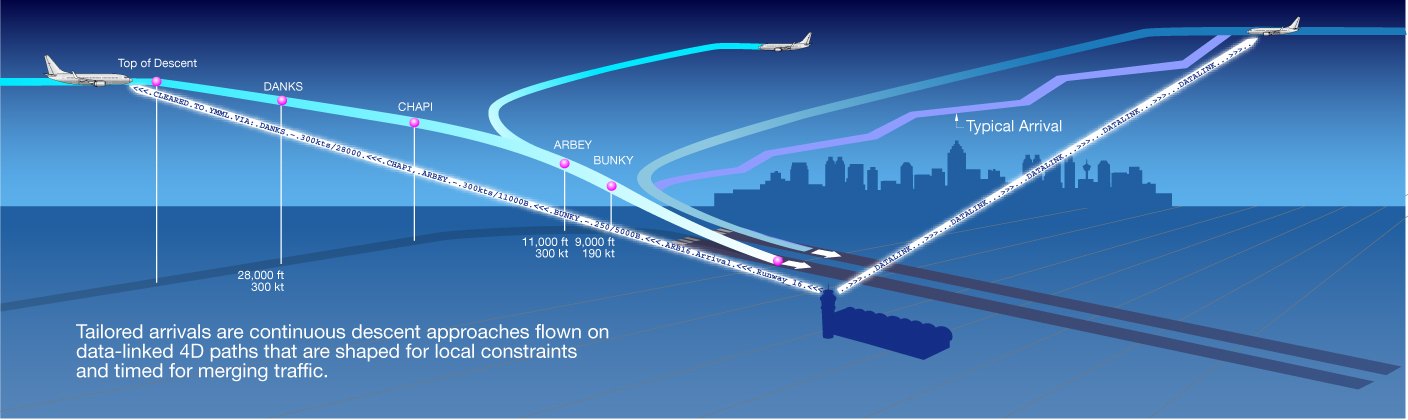
\includegraphics[width=1\textwidth]{figures/Tailored_Arrivals_YMML.jpg}
	\caption{Comparison of a STAR and TA profile at Melbourne International (YMML)}	
	\label{fig:Compare}
\end{figure}
\vspace{-0.8mm}
In the mid-1970s, British Airways began constant angle descents into Heathrow Airport, from an initial height of 7000 ft above ground level, mainly aimed towards noise reduction. CDA has been developed to begin from the cruise altitude, enabling a smooth profiled descent into the airport. CDAs are part of the larger Tailored Approaches (TA), the term more commonly used in the USA.\par
\begin{figure}
\centering
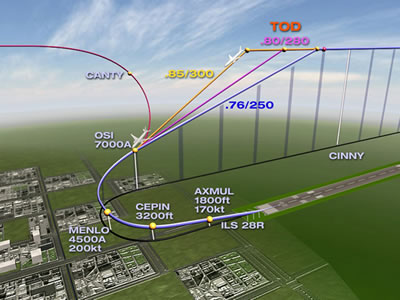
\includegraphics[width=0.45\textwidth]{figures/ils28R_tailored.jpg}
	\caption{A tailored approach into San Francisco International Airport (KSFO) Runway 28R}	
	\label{fig:KSFO ILS 28R}
\end{figure}
Major Airports that have implemented the CDA/TA include:
\vspace{-2.4mm}
\begin{enumerate}
\itemsep-0.5em
\item Los Angeles International (KLAX)
\item Heathrow International (EGLL)
\item Hartsfield-Jackson International (KATL)
\item San Francisco International (KSFO)
\item Louisville International (KSDF)
\end{enumerate}
\vspace{-2.4mm}
Some of the benefits as reported by Airlines that participated in the KATL study reported fuel savings of approximately \href{http://www.gtresearchnews.gatech.edu/continuous-descent/}{300-1000 pounds of fuel}. Since the CDA has a smooth glide profile, aircraft engines do not throttle up and down reducing the noise and emissions. Keeping engines at idle power can cut emissions of nitrogen oxides by nearly a third, and reduce noise along certain portions of the flight path prior to the Initial Fix point. CDA also has the benefit of being faster, saving a few minutes during the descent and landing phase of the flight.\par

Air New Zealand (ANZ) and QANTAS participated in the \href{http://www.airways.co.nz/documents/Aspire-Annual-Report.pdf} {ASPIRE} program, which aimed at having actual commercial flights that served as demonstrations  to set an "Ideal Flight" benchmark metric. On 12 September 2008 the inaugural test flight, an ANZ-operated Boeing 777 demonstrated the capabilities of the most advanced Air Navigation Services and airline fuel optimisation initiatives in current operation. This flight had all practical operational restraints removed: including air traffic congestion control vectoring, air traffic fixed route structure, procedures, flow restrictions and airline restraints. This flight had 3.5 tonnes fuel savings (11.2 tonnes $CO_2$ reduction). One month later Qantas flew a new A380 from KLAX -YMML saving 8.9 tonnes fuel (28 tonnes $CO_2$). Although idyllic, these flights served as a benchmark for achievable savings, to which CDA contributed. \par

%%===================================================================================================================
\section{Case Studies Summary}  \label{sec:case studies}

This report analyses the works of several researchers as listed out in the bibliography. In specifics:
\begin{itemize}
\item Park and Clarke \cite{Park:2015} look at the performance bounds of CDA procedure via optimal vertical trajectory generation problems with respect to flight time and fuel consumption. Using two different types of aircraft (Boeing 737 and Boeing 767) in a numerical study, they compare the optimal CDA trajectories with a typical vertical navigation (VNAV) CDA trajectory used in CDA applications at several airports. They divide the optimal CDA vertical profile into two segments: the cruise segment before the top of descent (TOD) and the descent segment from the TOD. The descent section is further subdivided based on flap setting and speed constraints. 

\item Cao et al \cite{Cao:2013} Approach this topic from the perspective that studies which examine fuel savings from CDA
fail to consider the increased separation uncertainties that it often necessitates. They mention that this may cause extra
fuel consumption for safe spacing. Their study evaluates the fuel benefits of CDA at Atlanta Hartsfield-Jackson Airport taking into account the delays resulting from conflict resolutions. They estimate fuel burn using a corrected Thrust Specific Fuel Consumption model that is designed specially for descent. Conflict-free CDAs are determined in such a way that the total arrival
delays are minimized in each look-ahead time window. Resultant delays are converted to speed advisory or air holding commands executed in cruise phase to account for the impact of increased separations in CDAs. The fuel consumption of CDA is compared with that of real step-down trajectories extracted from radar track data. 


\item Jin and co-authors \cite{Jin:2013} also focus on the evaluation of the continuous-descent approach as a fuel-reduction procedure. Their research gives insights into the reasons why the continuous-descent approach saves fuel, and they derive design guidelines for the CDA procedures based on fuel burn dependency on speed and altitude. Their basis is the theoretical analysis that speed profile has a substantial impact just as important as vertical profile on the fuel consumption within the terminal area. In addition, the CDA is not intrinsically a fuel-saving procedure: it is contingent on conformity to the speed schedule. Based on this model, the potential fuel savings due to the CDA at the San Francisco International Airport (KSFO) are estimated, and the accuracy of this estimation analysed.

\item Mur\c{c}a and M{\"u}ller \cite{Murca:2015} present an optimization approach for dynamically scheduling aircraft operations and supporting air traffic controllers in both determining and implementing operationally feasible landing and departure times at an airport. They use a programming model to incorporate air traffic control infrastructure in terms of route network. Their model also introduces the concept of alternative approach routes and is designed to generate an output that can be converted into effective advisories for executable flight commands. It shows reasonable computational times for obtaining the optimal solution and delay reductions of up to $35 \%$ with practical size instances from Sao Paulo/Guarulhos International Airport (SBGR).

\item Takeichi and Inami \cite{Takeichi:2010} discuss the arrival-time controllability of the tailored arrival paths determined by the top-of-descent and waypoint positions. They consider a tailored arrival path which is designed using the least number of track-to-fix and radius-to-fix legs neglecting the engine thrust. They investigate two types of tailored arrival paths; one determined by adjusting the waypoint positions with the fixed top of descent, and the other determined by top-of-descent position with the fixed waypoints. These are numerically analyzed so as to satisfy a set of appropriate boundary conditions both at the top of descent and landing, and the behavior of the arrival-time difference from the standard continuous descent approach path is explored using a representative set of inputs. The arrival-time controllability is defined as the differences between the fastest and the slowest arrival time. Through several series of arrival-time analyses, it is found that the tailored arrival paths determined by changing the waypoint positions can achieve the larger arrival-time controllability compared with those determined by changing the top-of-descent position. It is also suggested that it is possible to compose an arrival path with the maximum arrival-time controllability without any additional fuel consumption.


\item Turgut et al \cite{Enis:2010} analyze the impact of CDA on fuel consumption, noise and emission.


\item Cao, Rathinam and Sun \cite{Cao:2011} present a rescheduling method for solving the conflicts between arriving aircraft which fly their preferred descent paths using the continuous descent approach. Their work is based on the 4-D trajectory concept: each aircraft calculates its 4-D trajectory and the Estimated Time of Arrival before initiating descent procedure, and reports the 4-D trajectory to the terminal area controllers at the destination airport. The reported 4-D trajectories are used for arrival sequencing. The objective is to minimize the total delay while keeping the inbound traffic conflict-free. The rescheduling problem is formulated as a Linear Program and solved with a solver, which provides as a solution the delay assignments which aircraft use to adjust the arrival time for conflict avoidance. A minimum in-trail separation is imposed between successive arrivals to meet the arrival rate of the airport. Their proposed approach leads to a conflict-free inbound traffic. Most importantly, it benefits the continuous descent approach in a sense that the conflicts are solved without changing the user-preferred trajectories, and the CDA trajectories are keep intact. 


\item Coppenbarger et al \cite{Copp:2007} discuss operational trials that were completed in January 2007 involving trans-pacific flights into San Francisco during early morning hours. Trajectory-based clearances were transmitted by data-link to Boeing 777 aircraft equipped with Future Air Navigation System avionics. NASA’s prototype, ground-based automation for high-density arrival management tailored trajectory clearances to accommodate artificially imposed metering constraints. 

\item Robinson and Kamgarpur \cite{Rob:2010} estimate the potential benefits of continuous descents for more than 480,000 flights to 25 major airports in the U.S. National Airspace System. While reduced fuel consumption and greenhouse gas emissions are expected for these procedures, the benefits during periods of congestion are not well understood. To address this gap, they constructed baseline trajectories  from flight plan and track data for flights arriving at 8 busy terminal areas. They modeled two types of continuous descent trajectories: One enforcing a constant distance-to-fly constraint to simulate decongested operations, while the other enforcing a constant time-to-fly constraint to simulate congested operations. They calculated potential fuel savings for different continuous descent scenarios. 

\item Nikoleris and co-authors \cite{Niko:2012} compare fuel consumption of alternative descent trajectories (from cruise altitude to meter fix) when the required time of arrival is later than the nominal time of arrival at the meter fix. The required delay, i.e. the difference between the nominal and the required times of arrival, can be achieved by either slowing down the aircraft in the cruise and descent phases or flying a longer route at a constant altitude. Performance models for ten different Boeing and Airbus aircraft, were obtained from Base of Aircraft Data, and used to generate results. 

\item Hayashi et al \cite{Hayashi:2011} propose an Efficient Descent Advisor (EDA) as a ground-based decision-support tool for Air Route Traffic Control Center (ARTCC) sector controllers for managing arrival flows. This work is based on Coppenbarger et al \cite{Copp:2010b} Their tool calculates the maneuver instructions for an arrival flight to fly a conflict-free (when able), fuel-efficient, continuous-descent trajectory and also meet a time-based metering requirement at the Terminal Radar Approach Control (TRACON) boundary. As of the time of writing of their paper, speed variations and path-stretch maneuvers were the only degrees of freedom used by EDA to find a solution. Their study examined the feasibility of altitude change as an additional degree of freedom. 

\item Alam and co-authors \cite{Alam:2010} investigate the benefits of CDA with change in traffic conditions and variable noise abatement rules and consider throughput capacity of transition airspace for multiple flights performing CDA operations.


\item Coppenbarger et al \cite{Copp:2010b} present an overview of development and testing of ground-based automation for accommodating fuel-efficient arrivals in heavy traffic, this work serves as a foundation for Hayashi and co-workers\cite{Hayashi:2011}. They define the Efficient Descent Advisor (EDA), an emerging decision-support tool for air-traffic controllers managing arrival airspace in enroute facilities. It generates trajectory-based clearance advisories that allow a continuous descent at low engine power while avoiding conflicts and maximizing arrival throughput. Findings from several human-in-the-loop simulations and a field test are presented and discussed, which pertain to controller use and acceptance of EDA as a near-term capability for the Next-Generation Air Transportation System (NextGen).

\end{itemize}


%%===================================================================================================================
\section{Methodology} \label{sec:methodology}

This section contains a summary of the case studies referered to in \ref{sec:case studies}:

\begin{itemize}

\item Park and Clarke \cite{Park:2015} 

This concern may be addressed by computing the required minimum separation between aircraft performing a CDA. Ren and Clarke developed the tool for analysis of separation and throughput for this purpose, and demonstrated its utility via flight test. Another approach to handle the throughput issue in TRACON is to assign a required time of arrival (RTA) at a meter fix for each aircraft. The RTA assignment at a meter fix requires a CDA performance-bound analysis of individual aircraft for the feasible operation. For this reason, ATCs need a methodology to analyze the performance bound of the CDA trajectory depending on the aircraft types and wind conditions. An optimal control framework is useful to analyze the performance bound of the trajectory. Therefore, to maximize the benefits of the CDA procedure and to study the performance bound of a CDA trajectory, we develop and examine the trajectory optimization of the CDA procedure in the optimal control framework. Several methods have been proposed for trajectory optimization. Erzberger and Lee [6] proposed a trajectory-optimization scheme for a fixed range in terms of direct operating cost, which is the combined cost of fuel and flight time. Sorensen and Waters [7] proposed an airborne fuel optimal flight-trajectory-generation method to meet the assigned time of arrival. Burrows [8] proposed an onboard fuel optimal-trajectory-generation method for fixed-time and fixed-range flight. Chakravarty [9] proposed a fuel optimal en route descent trajectory, including the cruise segment. In these studies [6–9], simplified energy state equations that use energy as the independent variable instead of time were used as aircraft dynamics equations, reducing the problem size. However, operating requirements, such as flap
extension and speed limits, were ignored. Visser and Wijnen [10] described a multiphase optimal control problem with respect to community noise impact in the vicinity of airports. In this research, optimal results were obtained for aircraft operations below 10,000 ft by using awakening as a performance index. Slattery and Zhao [11] proposed a trajectory-synthesis method with a predetermined sequence of vertical area navigation (VNAV) functions for the enroute descent phase by using their own capture-condition analysis of each VNAV mode [12]. However, this trajectory is not optimal. In this paper, we present optimal CDA trajectories that maximize the benefits in terms of operating costs, such as fuel consumption or flight time. The performance bound of a CDA trajectory is determined by the two optimal trajectories [13]. Idle power is assumed during the descent. To obtain these optimal trajectories, we formulate problems as multiphase optimal control problems with a fixed range, and consider both operating conditions and speed constraints. The altitude range considered in this paper is from the cruise altitude to the intercept of the Instrument Landing System (ILS) glide slope. By dividing the optimal trajectory into two flight segments, cruise and descent, we simultaneously obtain both the position of the TOD and the subsequent optimal descent path. Furthermore, we propose suboptimal trajectories for a VNAV CDA based on the optimal-trajectory results. The proposed VNAV CDA vertical profiles can be calculated by an onboard flight management system (FMS) computer without additional equipment, and the numerical results show that the performance of the proposed profiles is very similar to the optima


We simulate two aircraft types, B737 and B767, with pre-
determined flap-speed schedules. In the simulation, the altitudes are
specified relative to the mean sea level, and the airspeed constraints in
Sec. II are given as CAS instead of IAS. We assume that CAS is
equivalent to IAS by ignoring the installation error. The aircraft
performance data from the base of aircraft data (BADA) [16] are used
in the analysis. However, other general performance data can be used
because the formulation is quite general. The predetermined flap-
speed schedules are shown in Table 1. The aircraft mass chosen is
52,000 kg for the B737, and 158,800 kg for the B767 based on
BADA.
We choose the boundary condition for the numerical examples
based on the CDA flight test in Louisville International Airport
(KSDF) in [2]. We select a cruise altitude of 35,000 ft and a cruise
speed of Mach 0.7818 (265 kt). The maximum allowable descent
speed is 350 kt for both B735 and B764. As shown in Table 2, the
trajectory optimization starts at the chosen cruise altitude and cruise
speed, and terminates at the IAF with an altitude of 3000 ft at a track
distance of 8 n mile from the runway threshold and a speed of 180 kt.
After this point, the aircraft captures the ILS glide slope and flies
the ILS approach. The d max is set as 150 n mile for both the B735
and the B764. The International Standard Atmosphere conditions
are assumed for this simulation, and the air density, pressure, and
temperature equations in [16] are used.

We also compare the optimal trajectories to a reference CDA
trajectory generated by the FMS VNAV function. This vertical
trajectory was used for a flight test conducted at KSDF in
September 2004 [5]. As shown in Fig. 3, the KSDF VNAV CDA
profile is determined by a series of VNAV modes. The first segment of this trajectory is the cruise segment. The second segment of the
VNAV CDA profile is the idle-thrust segment. In the second segment,
the en route part, which is above 10,000 ft, is generated by constant
Mach, constant CAS, and constant descent-rate modes [22]. In the en
route part, constant Mach/CAS is set to 0.7818/350 based on the
KSDF flight test. At the end of the en route part in the second
segment, the aircraft attains the FAA regulated speed of 250 kt at
10,000 ft. From that point onward, constant CAS at 250 kt and
constant FPA segments are used to satisfy the final-point conditions.
The VNAV CDA profile is calculated via backward integration from
the final point to the TOD. The mode change between the constant
CAS and the constant FPA occurs when the CAS reaches 250 kt
during the backward integration from the IAF. By this way, the engine
throttle would remain at idle during the entire procedure from the
TOD to the final point.


\item Cao et al \cite{Cao:2013} 
This research relies on high fidelity simulation. The baseline in this study is the radar
track trajectories, which comes from FAA Performance Data Analysis and Reporting System
(PDARS). The data contains flight information, such as 4-D trajectories, flight plans, arrival fix
and ground speed. Fig. 1(a) shows the ground tracks of arriving aircraft into ATL throughout a
full day’s operations for October 1, 2011. Subfigure B shows the Standard Terminal Arrival
Routes (STARs) that transit the arriving aircraft from Air Route Traffic Control Center airspace
to the TRACON airspace. Approximately 85% of arrivals follow STARs. ATL is chosen for this
research for two reasons. First, ATL has wide open airspace. The inbound traffic enters the ATL
terminal airspace through four corners. The arrival routes have a radial treelike structure. As a
result, interactions between arrival flows are minimized, which make it easier for deconfliction
modeling. Second, ATL is a hub airport that accommodates a large volume of traffic each day. A
large sample size improves statistical significance of the data analysis. TABLE 1 lists the
PDARS data used for CDA analysis.
Trajectories observed from the PDARS data mostly use conventional step-down descent.
To create CDA traffic, aircraft type specific information as well as ground tracks are fed into
FACET to synthesize CDA trajectories. FACET uses built-in aircraft performance data derived
from BADA to propagate the vertical profile of a given aircraft type, which is typically a 3
degree glide path. The lateral path is determined by waypoints derived from either flight plans or
a given geographic coordinates array. Figure 2 shows a sample step-down trajectory and the
corresponding CDA version simulated by FACET. Their ground tracks are exactly the same,
with only different vertical profiles. This is to ensure that the fuel consumption difference
between CDA and the baseline is only a consequence of optimized vertical profiles and speed
profile. The radar updates the aircraft position with an interval of around 1 minute. To obtain a
finer resolution, the update interval is turned to 5 seconds in FACET SIMULATION mode. The
simulated trajectory is a smooth glide path with delayed Time Of Descent (TOD) point.

Simulation Models: Fuel Model, Deconfliction Model, Speed Change and Air holding


\item Jin and co-authors \cite{Jin:2013} 
  This paper is organized as follows. Section II reviews some
previous research. In Sec. III, an analytical link between flight
operation parameters and fuel consumption is derived based on
the base of aircraft database (BADA) total-energy model (TEM),
resulting in some guidelines for the CDA design. Based on the results
from Sec. III, Sec. IV presents a case study at the San Francisco
International Airport (SFO), in which the macroscopic fuel savings
are estimated. Remarks and comments are provided in Sec. V.

   In this section, the analytical relationship between procedure
variables (vertical profile and speed profile) and fuel consumption
is derived. The fuel consumption is expressed as a function of
the vertical profile and the speed profile, which is fundamentally
nonlinear. Such nonlinearity will produce some nonintuitive effects,
for instance, elevation of flight level, increasing fuel consumption.
The results from this derivation will be applied to two special cases to
provide insights into fuel consumption in the terminal area, and to
explain the reason why the CDA typically reduces fuel consumption.




\item Mur\c{c}a and M{\"u}ller \cite{Murca:2015}
    As described before, the problem of aircraft sequencing and scheduling for landing is analyzed through an optimization
approach in this work. Since each aircraft has to perform a specific approach route to arrive at the destination airport (STAR),
 he model proposed attempts to encompass part of the associated control problem taking into account these arrival routes.
More specifically, a mixed integer linear programming model was developed, which seeks to minimize the cost of the devi-
ation of the actual landing time from the target landing time in determining how each aircraft will perform the arrival route
 o the airport so that the separation between aircraft on final approach is guaranteed. In other words, the model determines
 he discrete delays or time advances associated with alternative arrival routes and/or holding procedures that must be
 mposed to each aircraft in order to avoid a conflict. It is interesting to observe that the idea of this mathematical program-
ming modeling is similar to the airspace structure designed by Andreussi et al. (1981) in their fast-time simulation model.
They considered alternative approach routes from the feeder fix to the runway which generated delays with a range of one to
five minutes in order to organize the traffic flow.
    A STAR usually consists of a fixed number of waypoints and routes linking these waypoints. So, the landing time of an
aircraft is the time it passes over the first waypoint of the STAR plus the time spent to traverse the whole arrival route.
We considered that the time spent to traverse the STAR is the sum of the standard time spent if a continuous descent
approach is performed with discrete delays or discrete time advances resulting from controllers’ actions to guarantee the
 egulated separation between aircraft. These discrete delays or discrete time advances are associated with either alternative
arrival routes or holding procedures that can be performed by an aircraft. The type of the arrival route and the number of
holding procedures are a controller’s decision that impacts the landing time and that is what we aim to optimize.
    Here the major difference of the model proposed in respect to the model of Beasley et al. (2000) is noticeable. While the
 anding times are continuous decision variables in their model, in the model proposed they result from discrete decision variables associated with how an aircraft will perform the approach to the destination airport. Thus, there is a broader flow
management conception in terms of implementation, which can even be complementary to a management conducted out-
side the terminal area.

    The sequencing and scheduling decisions are made in a dynamic environment where the set of aircraft that are going to
land or takeoff and the set of aircraft that has already landed or taken off are constantly changing during the time. This on-
line process has two aspects of dynamics. First, the set of aircraft that the controllers have to schedule changes as time
passes, in other words, all the flights to be scheduled are not previously known as they would be in the static case. Second,
a previous scheduling decision can be updated as time passes and new aircraft enter the scheduling window such that the
rescheduling potential is higher for those aircraft that are farthest from the runway. Therefore, it is necessary to link the ana-
lytical model with a dynamic approach so that it can be better evaluated and become useful in a real time situation. In this
work, we developed a dynamic approach for running the optimization model that is based on the concepts of scheduling
window and freeze horizon described in Section 2.
    In our proposal, the scheduling window and the freeze horizon are time based. We considered a scheduling window that
is constantly updated at a rate that is equal to 60 min divided by the length of the freeze horizon. For a freeze horizon of x
minutes, we considered that the length of the scheduling window is 3x minutes and it is characterized as follows: the sched-
uled time of arrival at the airport for the flights that have estimated time of arrival within the first x minutes of the sched-
uling window is frozen and the arrival time at the airport for the flights that have estimated time of arrival within the last 2x
minutes of the scheduling window can still be scheduled (optimized). For every x minutes, the scheduling window is then
updated, encompassing a new set of aircraft with frozen scheduled time of arrival and a new set of aircraft with arrival times
to be scheduled. Therefore, we ensure that if a plane begins the arrival route within a time window and lands within the next
time window, it will be considered in the scheduling of the next sequence of aircraft. It means that the upstream flow and the
downstream flow will always be considered for scheduling and that separations will be ensured for all the pairs of aircraft.
Fig. 1 summarizes the dynamic approach proposed.
    It is important to discuss how this dynamic approach could be used in practice as part of a decision support tool for air
traffic controllers. For this, the processes that would happen during an optimization run will be described. First, for all the
flights between x and 3x minutes from the reference waypoint (fraction B and C of Fig. 1), estimated time of arrival (at the
final waypoint of the STAR) would be generated from a set of input parameters such as wind and speed profiles. This pre-
diction could be made either with the information of the radar console at the air traffic control body or with the flight man-
agement system of the aircraft (in this case, the predictions could be transmitted to the air traffic control body via data link).
Second, the model input parameter represented by the target time of arrival at the final waypoint of the STAR would be
updated by the values determined in the first stage. The scheduled time of arrival of the flights within the first x minutes
of the scheduling window (fraction A of Fig. 1) would also be updated with the results of the previous optimization run.
Third, the optimization procedure would be initiated. Once the results of the model are generated, in other words, the con-
figuration of the STAR to be traversed and the number of holding procedures to be performed, they would be displayed to the
air traffic controllers. Finally, with this information, the air traffic controllers would be able to transmit the appropriate con-
trol instructions to the next set of aircraft (fraction B of Fig. 1), which becomes the frozen fraction of the next scheduling
window (their scheduled time of arrival are frozen in the next optimization run). Here it is noticeable the benefit of the out-
put type of the proposed model in terms of decision support. Since the scheduled time of arrival is displayed in terms of con-
trol actions, air traffic controllers are supported not only in the establishment of an arrival sequencing and scheduling
solution but also in the implementation of this solution.
3.3. Case study
    The optimization approach proposed was analyzed with practical instances from Sao Paulo/Guarulhos International Air-
port (SBGR) – the largest Brazilian airport and an important hub in Latin America. It recorded 284,184 aircraft movements
and 35,962,000 passenger movements in 2013. SBGR has two parallel runways, one with 3000 m of length (09R-27L) and the
other with 3700 m of length (09L-27R). Due to the wind regime, the runway threshold 09 prevails for operations. The runway
09R-27L is usually used for landings while the runway 09L-27R is usually used for takeoffs. Since they are separated by
375 m and there is a displacement threshold of 580 m, the operations of arrivals and departures are dependent. It means
that departure flights need to be taken into account in the arrival sequencing and scheduling process.
    Real radar data from a typical day of operations (December 07, 2010) were used to perform the analysis in this work. Fig. 2
shows a plot of real SBGR flight trajectories (in blue) at this day of operations, when there were a total of 747 aircraft oper-
ations. The configuration of the STAR of SBGR is plotted in red (from each IAF to the airport) so that it is possible to analyze
the traffic behavior during the approach. It is noticeable the range of control actions used by the air traffic controllers for
sequencing and scheduling the arrival flights. Fig. 2(A) and (B) show two parts of the arrival route with zoom. It is possible
to observe that shortcuts and lengthened paths are very used by the controllers to provide the separation between aircraft.
For instance, in Fig. 2(B), it is possible to observe holding procedures at waypoints W1, W2 and W3, shortened paths from
W2 to W4 (without overflying W3) and lengthened paths from W1 to W4, revealing some of the actions that were probably
taken by the air traffic controllers to ensure the separation between aircraft at W4. Similarly, in Fig. 2(A), where it is given a
zoom of the final approach, there is a high dispersion before arriving at W12, with many shortened paths from W6 to W8
(without overflying W7) and several lengthened paths from W7 to W8. It is important to mention that it is reasonable to
assume that the deviations of trajectories shown in Fig. 2 are mainly because of air traffic control interference and not
because of imprecision of flight navigation. First, the geometric profile of actual trajectories shows deviations that are much
higher than the current level of precision in navigation and that clearly reveal a deterministic change in the trajectory. Sec-
ond, in the current stage of technological development, aircraft have been able to fly very precise routes with the introduc-
tion of Global Navigation Satellite Systems and Performance Based Navigation, both in use at SBGR flight procedures.





\item Takeichi and Inami \cite{Takeichi:2010} use the equations of motion to analyse the aircraft profile in the descent trajectory by performing a flight path composition comparison for standard descent as well as CDA. They then use these equations to evaluate the arrival time for various flight angles which incorporate a given approach of a certain angle towards the base leg of the flight approaching the runway. They then calculate fastest arrival times and paths that will enable this.



\item Turgut et al \cite{Enis:2010}
Conventional and CDA procedures were modelled in the Istanbul terminal area (TMA), which has five entry points. The real speed and the real altitude limitations were maintained on these entry points. System for Assessing Aviation’s Global Emissions research results were also used to determine the emission savings. This study was implemented for different approach routes to
the Istanbul TMA. Locating at 408580 56.4600 N and
288480 26.5500 E, International Istanbul Ataturk Airport has
been ranked as 16th according to the 2006 total departure
among the largest 25 European airports (Eurocontrol Trends in
Air Traffic, 2007). It is equipped with three configuration of
runways, so-called as 06/24, 18L/36R, and 18R/36L. Most used
configuration of runway is a06/d36, which the statistics in 2000
states that this runway (arrivals on RWY 06 and departures on
RWY 36) was used 60 percent of time, while the remaining 40
percent being on configuration a24/d18 (Eurocontrol
Assistance to Turkish State Airports Authority, 2002). For
this reason, the runway 06 was chosen for arrival airliners.
Furthermore, it has five entry points through the TMA. Entry
point names and their locations are given at Table I. The speed
maxima for entry points and for the final approach point (FAP)
are 250 and 210 kts, respectively. The required altitude at the
FAP points ended for the paths of all the entry points are
2,600 ft and the FPA is assumed as 38 throughout the study since
it is an optimum descent angle.
   In conventional approaches the profile between these entry
points and the FAP depends on the pilots as long as the
altitude and the speed restrictions do not be exceeded. For
the numerous approach cases, after the entry points the pilots
descend until the minimum altitude limits and proceed low-
level flights until the FAP. However, this approach leads more
fuel consumption and takes more time according to the CDA.
Furthermore, some entry points would let this kind of
approach with two steps as descent to 3,000 ft and level flight
at 3,000 ft, while for the others four steps stair approach is
required as two descents and two low-level flights.

According to the Table I, level flights altitudes between 8,000
and 12,000 ft instead of 3,000 ft (as being in the conventional
procedures) are proposed. The FPA from the entry points are
all-same for either approach procedures for an individual
flight profile except the two of them which have stepped
descent profile. Moreover, the level flight distances are also
same for either approach procedures. The single distinction is
the altitude of the level flight took place.
   This study is modelled for one single flight per entry point.
For this context, B757 was selected in order to demonstrate
the results of CDA procedures in terms of fuel consumption,
time and emission. It has two PW2037 medium by-pass
turbofan engines, which has 166.4 kN thrust each. Taking
into consideration that airliners can use various type of
engines, some flight data attributed for the case flights of the
airliner are listed at Table II.
   Table II involves four phases of flight as the names of takeoff,
climb out, cruise and descent. The main reason of the weight
reduction is the fuel consumption which equals 9.9 t and this
does not include the APU fuel which could be additional several
hundred kilograms (ICAO Airport Air Quality Guidance Manual,
2007). The fuel allocation share is calculated as 4, 21.2, 70.7
and 4 percent as the aforementioned order of the phases of
flight. The inequality of the sum of the percentages as 0.1
percent is due to the round-off error. Since it is a required
consumption, excepting the takeoff phase, both of climb out
and cruise phases are optimized for the minimum fuel
consumption as considering the optimum altitude. However,
despite relatively low share among the entire fuel consumption,
the descent phase has significant fuel saving potential in terms of
operation and traffic procedure.
   The fuel flow records represent ranges instead of absolute
values. The reasons could be listed as the changes in altitude
according to climb or descent and weight reduction result from
the fuel consumption on board, particularly in cruise. These
parametric changes have impacts over the fuel consumption
since the thrust demand should also be changed to offset the
required lift continuously and safely. In climb out phases,
increasing the altitude has positive effect over the engine
performance, which leads lower fuel consumption for the same
amount of thrust or the rate of climb. Moreover, almost
7,000 kg fuel usage reduces the required lift of the airliner and
the fuel consumption.
   Regarding to the engine pressure ratio (EPR) indicator,
which is used for the determining the thrust, the maximum
value occurred in the end of the climb out phase. Since the
EPR measures the ratio of the compressor inlet pressure and
the turbine outlet pressure, the ambient pressure is revealed as
an important factor. Therefore, high EPR at the end of the
climb out phase could be explained by having relatively high-
engine power and low-ambient pressure. Further focused on
EPR, provides an objective of the descent as minimum EPR
as sufficient to maintain the speed and glide path as possible
as. This minimum EPR leads also minimum fuel
consumption. As seen at Table II, lowering the altitudes
increase the EPR, since 0.741 and 0.917 denote the altitudes
of 37,000 and 3,000 ft, respectively. This objective is also one
of the supports to the general rule of “level flight at lower
altitudes leads more fuel and time consumption” (Tong et al.,
2007).
   The general altitude limits for splitting the phases referred
at Table II can be given as:
.
     takeoff – up to 3,000 ft;
.    climb out – between the 3,000 ft and the cruise altitude;
     and
.
     descent – below the 3,000 ft.
In order to distinguish the gains between conventional and
CDA procedures, one needs to obtain the airliner
performance for level flight at different altitudes, in
particularly lower than FL120, since the descent flight path
to 3,000 ft from the entry points altitudes are same. Hence,
Base of Aircraft Data (BADA) performance table of B757
is used for the level flight performance data (Eurocontrol,
2004). Moreover, since these performance parameters
(i.e. both the real flight data logs and the BADA) are
recorded for calm wind conditions, the wind impacts are not
taken into consideration throughout the study.
   Up to now, we discussed the traffic and the operation
perspectives of the methodology. After providing the area,
entry points, airliner, and the other flight data, it is required to
determine the emission values produced from both
conventional and CDA procedures. However, there is no any
absolute model about determining the actual amount of
emission that completely agreed since the fuel consumption
depends upon numerous uncertain parameters including
weight, weather, operation, traffic, etc. besides the other
certain parameters such as cruise altitude and range.
Therefore, for this study the model is selected in such a way
that could be able to cover wide range of engine and airliner
types.
   In this context, with a project implemented by FAA and the
other partners, System for Assessing Aviation’s Global
Emissions (SAGE), wide range data dealt with emission
impacts of aviation were gathered together for the years from
2000 to 2004. These data are also classified due to the
airliner, engine, country, region and, etc. within that project.
Besides, the SAGE, one of the other emission databases,
ICAO engine database was also used where SAGE values
needed to be checked at some part of the study.


\item Cao, Rathinam and Sun \cite{Cao:2011} 
Their work is based on the 4-D trajectory concept: each aircraft calculates its 4-D trajectory and the Estimated Time of Arrival before initiating descent procedure, and reports the 4-D trajectory to the terminal area controllers at the destination airport. The reported 4-D trajectories are used for arrival sequencing. The objective is to minimize the total delay while keeping the inbound traffic conflict-free. The rescheduling problem is formulated as a Linear Program and solved with a solver, which provides as a solution the delay assignments which aircraft use to adjust the arrival time for conflict avoidance.
    An ideal vertical profile of CDA is simulated using the Future ATM Concept Evaluation Tool (FACET)7
and shown in Fig. 1. The CDA keeps the aircraft cruising at a relatively high altitude as long as possible.
When arriving at the top of descent (TOD), the aircraft descends along a smooth slope with engines running
at idle or near-idle settings which require significantly less engine thrust. Compared to the conventional
step-down descent, the CDA reduces8 fuel consumption, emission, and noise impact by avoiding low altitude
(between 3,000 ft and 10,000 ft) level flight before intercepting the final 3 degree glidepath (normally 8 to
25 nautical miles away from the touchdown depending on local circumstances).9 It also saves flight time
due to the longer high altitude cruise with high speed. However, regardless of the environmental benefits,
to date the CDA has yet been a nationwide practice due to airport safety and efficiency concerns. The near idle throttle settings makes the descent trajectories less predictable. As a result, air traffic controllers
(ATCs) have to block large chunk of airspace to separate the landing aircraft. This leads to a reduction in
the throughput of an airport. So far, the CDA has been practiced only in low-density conditions or applied
to a selected portion of inbound traffic in the nighttime hours rather than on a standard terminal airspace
operation basis.8, 10–12     The 4-D Trajectory Based Operations is a concept that can enhance the predictability of the CDA.13
Essentially, in this concept, each aircraft has a capability to accurately follow a planned, feasible trajectory
that has been agreed upon with the controllers. The operations are then based on these trajectories that
specify the complete set of positions of each aircraft along with its time of arrival at each position. The
realization of this concept strongly depends on the on-board FMS and a reliable datalink between the aircraft
and ATCs.14 Aircraft equipped with the P-RNAV system is able to fly a 4-D trajectory accurately be within
+/-1 NM for 95% of the flight time.15 En route flights calculate its estimated time of arrival (ETA) and
planned standard terminal arrival routes (STARs), then report to the ATCs for approval via dedicated
datalink. ATCs send back the RTAs and STARs which help the FMS to fine tune the accurate ETAs. Such
negotiations are initiated at least one hour before reaching the TOD, allowing sufficient time for the ATCs
to sequence and merge the arriving flows. Their model has a conflict resolution model that is enabled.
The validation consists of two simulations. In the first simulation, aircraft perform unconstrained CDAs
without rescheduling. Each aircraft is navigated by the filed flight plans, and descends along the course of
CDA adhering to the built-in performance database. The first simulation generates the 4-D trajectories of
all flights. The conflict count obtained from this case serves as a baseline. In the second simulation, aircraft
perform constrained CDAs under separation constraints and airport arrival rate constraint. R is set to be
180 nm such that majority of the TODs lie inside the yellow circle in Fig. 4. As a result, majority of the
CDAs are not interrupted as delay controls are finished outside the terminal area. The 4-D trajectories
exported from the first simulation are fed into the re-scheduling algorithm. The MILP is solved by CPLEX.
Once the optimization is done, the optimal delay solutions are used to run the second simulation. In both
simulations, statistics of fuel consumption and flight time are recorded, as well as the conflict information.




\item Coppenbarger et al \cite{Copp:2007} 

     In collaboration with the FAA and United Airlines, The Oceanic Tailored Arrivals (OTA) trials were conducted
over 40 days with a single United Airlines Boeing 777 flight (UAL76) in commercial service between Honolulu and
San Francisco (SFO). The flight was operated along the Central-East-Pacific (CEP) oceanic route structure,
comprised of a series of fixed, parallel tracks from the Hawaiian Islands to the California coast.12 In addition to its
avionics equipage, UAL76 was chosen largely because of its early morning (5:30 AM local) arrival time at SFO,
which avoided congested airspace conditions, thereby minimizing the likelihood of interference with other traffic.
A. System Components
     Figure 1 illustrates the key systems employed in formulating, communicating, and executing the trajectory-based
arrival clearances used to support the OTA field trials (the precise content of the data communications between the
various system elements is described later in the paper). Clearance delivery was initiated approximately 700 nmi
from landing in oceanic airspace controlled by the Oakland Air-Route Traffic Control Center (ARTCC), referred to
as ZOA. In oceanic airspace, controllers at ZOA rely upon the FAA’s recently deployed Advanced Technologies
and Oceanic Procedures (ATOP) system for integrated CNS functions. A prominent capability of ATOP is its ability
to support two-way digital messaging between ATC and the flight deck through Controller-Pilot Data-link
Communications (CPDLC). The OTA route clearance – comprised of lateral waypoints together with speed and
altitude restrictions – was relayed to the flight deck using a standard CPDLC message format supported by ATOP.
The format allowed the OTA instructions, upon pilot approval, to be directly loaded into the B777 FMS through its
Future Aircraft Navigation System (FANS) avionics interface. FANS avionics integrate FMS functionality with
CPDLC and contract-based Automatic Dependent Surveillance (ADS-C) services in oceanic airspace.
    Once loaded, the OTA route clearance provided sufficient information for the FANS FMS to compute a 4-D
reference trajectory from the aircraft’s current position to the runway. This trajectory was then used by the FMS as
the basis for its Lateral Navigation (LNAV) and Vertical Navigation (VNAV) guidance functions, which provided
inputs to the automatic flight control system for determining appropriate aileron, rudder, elevator and throttle inputs.
Once activated, the OTA route clearance allowed the flight to progress with no additional pilot inputs required prior
to configuring the airplane for landing. The nominal guidance law used by the FMS VNAV function was set to
PATH mode, which directed the autopilot to null any positional error between the airplane’s current altitude and the
FMS reference trajectory’s vertical profile. In the event that the airspeed required to control path differed from that
suggested by the reference trajectory by more than ±10 kt, the VNAV guidance laws would switch from PATH to
SPEED control mode.
    To provide a dynamic element to the OTA trajectory-based clearance, a prototype version of NASA’s EDA
decision-support tool was incorporated into the field trials. EDA was used to compute the maneuver solution needed
to target a meter-fix crossing time constraint imposed at the Terminal Radar Approach Control (TRACON)
boundary. Originally designed to assist the domestic en route sector controller in developing conflict-free arrival
metering solutions under capacity constrained conditions, EDA was adapted to ZOA airspace and interfaced with
ATOP to receive oceanic surveillance and flight-plan data. This oceanic surveillance data was derived from the
airplane’s satellite-based positioning system, and relayed to ATOP via ADS-C at the maximum-available rate of
once every 2 minutes, as specified in the ADS-C contract configured by ZOA. In addition to surveillance and flight
plan inputs, EDA required atmospheric data to compute the long-range trajectory predictions needed for its
advisories. These input data were derived from the National Oceanic and Atmospheric Administration’s Rapid
Update Cycle (RUC) model, which provided 2-hour forecasts (updated each hour) of wind speed, wind direction,
temperature and pressure, organized in a Lambert-Conformal 3-D grid with a lateral resolution of 40 km.
    For the purpose of the OTA trials, EDA computed only descent Calibrated Airspeed (CAS) advisories for
targeting a Scheduled Time of Arrival (STA) at the TRACON meter fix (waypoint BRINY). EDA cruise-speed and
path-stretch advisory capabilities, along with automated conflict resolution functions, were purposely suppressed to
avoid complexity and unnecessary risk in these initial trials. For optimal TRACON throughput under congested
conditions, EDA derives its target STAs from TMA. During the time of these trials, however, no capacity
constraints existed, so meter-fix STAs were artificially set to within ±4 minutes of the airplane’s original Estimated
Time of Arrival (ETA) at BRINY. This original ETA was computed from an EDA trajectory prediction using a
nominal assumption of company-preferred descent speed (280 kt).11 An example of EDA’s graphical user interface,
    At Step 1 in Figure 4, the flight crew requested participation around 90 min prior to their estimated landing time,
approximately 700 nmi from SFO and 450 nmi prior to entering radar-controlled, domestic airspace. This request
was made using a free-text CPDLC datalink message that read “Requesting OTA trials.” Upon receiving the crew
request, the OC-4 controller configured a new ADS-C contract within ATOP that instructed the aircraft to downlink
position, weather, aircraft state, and flight-path intent data at a rate of once every 2 minutes, represented by Step 2 in
Figure 4.
    Following ADS configuration, the basic OTA clearance, as previously described, was up-linked to the aircraft
using a FANS-loadable CPDLC message (Step 3). The message, conveyed using CPDLC Uplink Message (UM) 83,
was as follows: “At COSTS cleared CREAN CINNY BRINY/N0240A110 OSI/N210A070 MENLO/A045A
ILS28R.” The test engineer coordinated with the ZOA-oceanic supervisor in advance to affirm the assumed landing
runway. Prior to accepting the clearance, the flight crew first ensured that it could be loaded satisfactorily into the
FMS to produce a continuous trajectory to the runway (Step 4). This FMS trajectory was computed in compliance
with the route, speed, and altitude constraints stipulated in the OTA clearance. Upon crew acceptance of the OTA
clearance, a “Wilco” message was downlinked to ATOP.
    Step 5 involved the uplink of wind and temperature data to the flight deck for inclusion in FMS trajectory
calculations. These atmospheric data were derived from the same RUC 2-hour forecast model used for ground-based
EDA trajectory calculations. In addition to the forecast surface temperature at SFO, the data consisted of wind
speed/direction at five points along the OTA trajectory corresponding to 1) cruise altitude at the waypoint CINNY,
2) cruise altitude at TOD, 3) 18,000 ft along the descent path, 4) 10,000 ft along the descent path, and 5) threshold
crossing at SFO. These data were uplinked to the flight deck to provide FMS trajectory computations with the same
atmospheric data available to EDA. This was essential to make valid trajectory-prediction comparisons between
ground-based and airborne automation in post-trial analysis.
    Step 6 involved the uplink of the EDA descent-speed advisory, intended to control arrival time at the waypoint
BRINY. The advisory was obtained from a prototype EDA tool running on a laptop computer in the ZOA-Oceanic
control room. Upon extracting the advisory, the test engineer relayed it to the oceanic sector controller managing
UAL76. The controller then used ATOP to relay the instruction to the aircraft in a datalink message consisting of
current Mach number and the advised descent CAS. Upon receipt by the flight deck, the descent speed instructions
were manually entered into the FMS VNAV descent page, which resulted in a recalculation of the FMS TOD and
trajectory needed to target the BRINY constraint. Once reaching TOD, the FMS commanded the airplane to initiate
the descent at an airspeed equal to the current Mach number until capturing the EDA-advised descent CAS.



\item Robinson and Kamgarpour \cite{Rob:2010} 
    This research estimates the potential fuel savings of continuous descents for more than 480,000 flights. Arrival
flights to multiple airports in multiple TRACONs were analyzed in order to encompass congested metroplex
environments, like New York, as well as super-hub environments, like Atlanta. The traffic analysis was performed
using NASA’s Center/TRACON Automation System infrastructure in conjunction with ARTCC and TRACON
flight plan and track data.16 The Aviation Systems Division at NASA Ames Research Center has 24 hour-a-day, 7
day-a-week access to the following data:
    • flight plan and track data for all 20 ARTCCs, as well as 27 TRACONs in the NAS,
    • NOAA Rapid Update Cycle (RUC) weather forecasts, and
    • NWS Meteorological Aviation Reports (METAR).
    Fuel flow analyses were performed using BADA and several Aircraft Operating Manuals. The results were
imported into an SQL data warehouse in order to investigate the macroscopic factors that strongly affect vertical
flight path efficiency. The potential fuel savings were aggregated by airport, arrival procedure, landing runway,
aircraft weight-class, and traffic demand level. More than 2000 CPU hours were spent processing the raw data on
high-performance Apple™ computers. The volume of the resulting data warehouse exceeded 1 terabyte of raw,
processed, and database-resident data.
A. Scope of Study
    The vertical flight paths were analyzed for arrival flights into 8 TRACONs in the NAS, including all seven so-
called Large, or Consolidated, TRACONs. The seven Large Level 12 TRACONs are Atlanta TRACON (A80),
Chicago TRACON (C90), Dallas/Fort Worth TRACON (D10), New York TRACON (N90), Northern California
TRACON (NCT), Potomac TRACON (PCT), and Southern California TRACON (SCT). The vertical flight paths
for arrival flights into Denver TRACON (D01) were included for comparison to Ref. 13. Arrival flights to these
eight TRACONs’ OEP 3517 airports, as well as to their major satellite airports, were analyzed. Table 1 summarizes
the traffic statistics for these facilities.



\item Nikoleris and co-authors \cite{Niko:2012} 
    Over the last two decades, a substantial amount of research and development has been done in the United States
and Europe to develop decision support tools for controllers to improve safety and efficiency of terminal area
operations. A notable example is the Traffic Management Advisor (TMA) that was initially developed at NASA
Ames Research Center as one of the Center-TRACON Automation System (CTAS)1 suite of tools. TMA technology
transfer to the Federal Aviation Administration (FAA) led to the development and deployment of the operational
version of TMA that is currently used for arrival management at major U. S. airports. TMA computes estimated time
of arrival (ETA) to the outer meter arc, meter fix, final approach fix, and runway threshold for each aircraft in the
arrival stream. ETAs of the aircraft are used to determine the required times of arrival (RTA) based on sequencing
and scheduling constraints. Advisories are then issued by the controller to the pilot to either slowdown or speedup in
order to arrive at the control point, such as a meter fix, at the time stipulated by the RTA. The Efficient Descent
Advisor2-4 (EDA), developed at NASA, generates maneuver advisories that allow controllers to achieve TMA-
derived RTA objectives while keeping aircraft separated. EDA provides speed, altitude and heading advisories that
can be easily followed by aircraft equipped with a Flight Management System (FMS) to meet an RTA. Depending
on the amount of delay, several solutions are possible as discussed in Ref. 2. Although EDA has been shown to save
fuel in comparison to today’s operations in which controllers have no automation for meeting RTAs, research that
attempts to rank a broad variety of trajectory types and delay-absorption strategies based on fuel consumption has
been limited. Several studies such as in Refs. 5 through 7 quantified fuel savings from implementation of continuous
descent approaches to an airport. These studies, however, did not seek to determine the most fuel-efficient way for
conducting continuous descent to meet an RTA, but only to estimate the benefit of descents without an intermediate
cruise segment.
    The principal contribution of this paper is a comparison of fuel efficiency for several standard descent
procedures with an RTA constraint at the meter fix. Computation of fuel-optimal trajectory is not the objective of
this study. For a thorough study of the problem of determining fuel-optimal delay trajectories the reader is
referenced to Refs. 8 and 9. This current paper considers descent procedures as typically executed in actual
operations, which are not necessarily optimal from a strict fuel cosumption perspective. Thus, fuel burn results are
generated by simulating descent trajectories using Base of Aircraft Data (BADA) version 3.9 (see Ref. 10)
performance models of popular Boeing and Airbus aircraft with specified descent procedures such as speed
reduction, intermediate altitude, path stretch and fixed flight path angle. Delays ranging from 10 seconds to seven
minutes are examined. In all scenarios, the aircraft is initially at an altitude of 35,000 feet and at a distance of 150
nautical miles from the meter fix. Each scenario is characterized by the amount of delay that needs be absorbed and
the descent procedure used for absorbing that delay.


\item Hayashi et al \cite{Hayashi:2011}
 A. Airspace and Traffic
    For the human-in-the-loop simulation experiment, the Northeast arrival traffic flows into the Denver
International Airport were simulated. The flights went through high Sectors 09 and 16 and low Sector 15 of the
Denver ARTCC (ZDV) and were eventually handed off to the Denver TRACON. See Fig. 4 for illustration. Two
traffic flows, one via North Platte (LBF) and AMWAY, and the other via YANKI and Sidney (SNY), merged at the
SAYGE meter fix. The freeze horizon was located in Sector 09, approximately 190 nautical miles from SAYGE. A
set of hypothetical published EDA profile-descent restrictions called TELLR 1 Profile was used in the simulation.
    Two traffic scenarios were created by recording the live traffic data and modifying them, such as adding some
over flights to increase conflicts. Scenario 1 included 36 arrivals and 31 over flights, whereas Scenario 2 consisted
of 38 arrivals and 31 over flights. The arrival rate at SAYGE was 42 per hour in both scenarios to mimic a peak-time
traffic load. The peak instantaneous aircraft counts during a run were in the range of 14~22 in Sectors 09 and 16,
and 9~14 in Sector 15, depending on how the controller handled and handed off the traffic. The minimum horizontal
separation threshold parameters set in the conflict identification computation were 6 nautical miles for conflict
detection and 7 nautical miles for conflict resolution. The minimum vertical separation threshold parameters were
900 feet if both aircraft were in cruise or 2000 feet otherwise. The aircraft call signs were changed each time the
scenario was reused in order to reduce learning effects.
B. Participants
    Three ZDV controllers participated in the study, two of which were retired controllers. All three controllers had
participated in the previous EDA simulation experiments9 and were sufficiently familiar with the restrictions in the
simulated ZDV airspaces. The controllers switched sectors after each run in the order specified in the experimental
design (described later).
    On the flight-deck side, three instrument-rated pilots were recruited from the local northern California area. Each
pilot was assigned to a pseudo-pilot station for one of the three sectors, through which the pilot handled all the
aircraft in the sector and any handoffs from/to a neighboring sector. The pilot participants’ main tasks were to
conduct radio communications with the controllers and perform handoffs via the pseudo-pilot station. They did not
have to input the cleared EDA maneuvers into the FMS. The FMS was automatically uploaded, including
intermediate altitude maneuvers, when the controller pressed the ACCEPT button. Occasionally, the controller
issued non-EDA instructions, such as a heading, altitude, or speed change for separation. In that case, the pilot
manually input the instructed maneuver via the Mode Control Panel (MCP) or the FMS.
C. Simulator
    The simulation was conducted in the Crew-Vehicle Systems Research Facility at NASA Ames Research Center
in April 2010. Eight computers running Windows XP Professional x64 and three Linux-based computers were
networked for the simulation. Of the eight Windows machines, three were used for the sector controller seats, three
for the pseudo-pilot stations, one for both traffic scenario control and ghost pseudo-pilot station operations that
automatically managed all the traffic outside the three sectors, and one for audio data recording. CTAS was run on
the two Linux-based experimenter stations to control and monitor the EDA computation processes. The other Linux
machine was used for a ghost controller station, which, again, automatically managed all the traffic outside the three
sectors. Multi Aircraft Control System (MACS) software developed at NASA Ames Research Center12 was used to
emulate the user interface of the sector controller’s Display System Replacement radar-position (or the R-side)
workstation. The data-position (or the D-side) workstation was not included in this simulation. The three controller
seats were each equipped with a 2000 × 2000-pixel high-resolution BARCO monitor. Each controller was provided
with the same Cortron keyboard and trackball used at the ARTCC facilities. MACS was also used as the pseudo-


\item Alam and co-authors \cite{Alam:2010} develop a methodology to generate aircraft-specific dynamic CDA routes that are both laterally and vertically optimized on given objectives (noise, emission and fuel) from an Initial Approach Fix (IAF) to Final Approach Fix (FAF). The
methodology utilizes real-time aircraft position and defined objectives to generate CDA routes which can then be converted into a set of artificial waypoints for continuous descent in transition airspace. The methodology involves discretizing the terminal airspace into concentric cylinders with artificial waypoints and uses enumeration and elimination (based on aircraft performance envelope) from one
waypoint to other to identify all the possible routes. For each transition a variety of metrics including noise, emission and fuel burn were computed. From the resulting set of possible CDA routes, those routes are identified that represent the best trade-off on the given
objectives. One of these routes was then used to dynamically update the flight route for executing the CDA procedure. For noise they used the Overall Sound Pressure Level (OPSL) and for emissions they used four pollutants HC , CO , $CO_2$ and $NO_x$ . The dynamic CDA algorithm is implemented in a high-fidelity simulator ATOMS for Sydney Terminal Area with 34L as arrival runway for a Melbourne-Sydney flight (B737-400 aircraft, $CFM56-3C-1$ engines with a nominal weight of $58000 kg$). The dynamic CDA routes are then compared on noise, emission and fuel burn with same flight conducting a typical CDA procedure (MANFA ONE Arrival) at the Sydney airport (YSSY). They also incorporated a delay algorithm which used the flights' estimated time of arrival (ETA) at the IAF and then allocated them a conflict free CDA route by searching through available routes. The approach took into account the aircraft category and corresponding time occupancy at each artificial waypoint of the proposed CDA routes and propagated any delays back whenever conflict arose.

      In this paper we propose a methodology to
generate dynamic CDA routes. Dynamic CDA are
aircraft specific, starting from Initial Approach Fix to
Final Approach Fix. The word dynamic refers to the
fact that two aircraft in the same approach airspace can
follow two different trajectories: there is no standard
arrival (STAR); in practice, each aircraft will receive
its dynamic CDA by datalink before starting its
descent. These CDA trajectories are generated by
discretizing the terminal airspace into concentric
cylinders with artificial waypoints, and uses
enumeration and elimination (based on aircraft
performance envelope) from one waypoint to another
to identify all the possible routes. For each transition a
variety of metrics including noise, emission and fuel
burn are computed. From the resulting set of possible
CDA routes, those routes are identified that represent
the best trade-off on the given objectives.
      The proposed methodology is integrated into a
high fidelity air traffic simulator (ATOMS) [12]. The
methodology utilizes real time aircraft position and
defined objectives to generate trajectories which can
be converted into a set of artificial waypoints for
continuous descent in transition airspace for a given
set of objectives such as noise, emission and fuel
consumption.
      The dynamic CDA approach is developed with
consideration for future integration with Flight
Management Systems (FMS). To accommodate for
real-time updates to the lateral path, the algorithm
outputs a set of CDA trajectories with trajectory
change points (TCPs) which represent the possible
optimal trade-offs between competing objectives.
These CDA trajectories can then be displayed to the
approach/tower ATCs, where a controller can select a
solution based on operational preferences and uplink
the chosen trajectory to the aircraft.
      The proposed methodology is then extended to
multiple aircrafts scenario, by blocking the artificial
waypoints generated for the first aircraft and making
them inaccessible for other aircraft for a period of time
based on estimated time of arrival (ETA) of the first
aircraft at its respective artificial waypoints.



\end{itemize}





%%====================================================================================================================
\section{Results and Findings} \label{sec:results}



\begin{itemize}

\item FIX FROM HERE BELOW!

\item Park and Clarke \cite{Park:2015} 

C. B737 Results
The results of the B735 minimum-time and minimum-fuel optimal
trajectories are shown in Figs. 4 and 5 along with the VNAV CDA
trajectory. For the minimum-time case shown in Fig. 5, the aircraft
accelerates until it reaches the 350 kt maximum allowable speed, and
then descends at a constant CAS. To satisfy the FAA speed-limit
regulation, before 10,000 ft, the aircraft decelerates at the minimum
descent rate. Below 10,000 ft, the aircraft flies at the maximum speed
of 250 kt as long as possible before decelerating to reach the final
speed and altitude conditions. The altitude and speed profiles are
determined at the boundaries of several constraints. These char-
acteristics of the minimum-time profile imply that the aircraft flies
with maximum performance to reduce flight time.
The minimum-fuel trajectory is quite different from the minimum-
time trajectory. For the minimum-fuel trajectory, the aircraft flies
with idle power as long as possible; hence, the aircraft starts de-
scending much earlier than in the minimum-time case. From the TOD
to 10,000 ft, the aircraft descends with small variations in FPA, as
shown in Fig. 4. Furthermore, the speed variation from the TOD to the
end point of the first phase is also small. The speed profile is
determined to be near 250 kt, which is the maximum allowable speed
below 10,000 ft.
Figures 4 and 5 reveal an interesting result. At 10,000 ft, the
minimum-fuel and minimum-time trajectories intersect, and are
identical below 10,000 ft. This fact means that the noise impact is the
same for both optimal trajectories because the noise impact in the
vicinity of the airport is a function of the state of aircraft below
10,000 ft. Another important result is that the performance difference
between the minimum-time and minimum-fuel trajectories occurs
only above 10,000 ft trajectory, which is during the en route descent.
Table 3 reflects the numerical results of the optimal vertical
profiles for the B735. As shown in the table, the optimal TOD
position in the minimum-time case is 90 n mile from the runway
threshold, which is about 18 n mile closer to the runway threshold
than the optimal TOD for the minimum-fuel case, which is about
107 n mile from the runway threshold. In addition, if the aircraft flies
along the minimum-fuel trajectory, as much as 54 kg fuels can be
saved, which is about 11.88% of the total fuel burned in the
minimum-time case. On the other hand, if the aircraft flies along the
minimum-time trajectory, we can reduce flight time by 178 s, which
is a 12.16% reduction in the flight time compared to the flight time
needed for the minimum-fuel case. The VNAV CDA case results are
very similar to the results of the minimum-time case with a difference
in fuel burn of only 5 kg and a flight-time difference of only 20 s.
Because the minimum-fuel and minimum-time CDA trajectories
consist of the performance bound of the CDA procedure with a given
wind condition [13], ATCs or air carriers can improve their benefits
by varying the CDA trajectory between two performance limit
trajectories.
D. B767 Results
The optimal vertical and speed profiles of a CDA procedure for the
B764 with respect to minimum-time and minimum-fuel performance
indices are shown in Figs. 6 and 7, respectively. Compared to the
B735, the B764 is quite large and heavy; hence, the performance
characteristics of the aircraft are quite different from those of the
B735. Despite the large differences in the parameters, we can see that
the tendencies of the B764 optimal trajectories are very similar to
those of the B735 when comparing the trajectories and speed profiles
in Figs. 4–7. In the minimum-time case, the optimal CDA speed and
altitude profiles for the B764 are determined at the boundaries of the
constraints, and this tendency is the same as that for the B735 optimal
profiles. The minimum-fuel optimal profiles for the B764 intersect
the minimum-time optimal profile at 10,000 ft, and below this point,
the optimal profiles of two performance indices are the same as in the
B735 case. As in the B735 profiles, the noise impacts below 10,000 ft
are identical between the minimum-fuel and minimum-time
trajectories.
The numerical values of the optimal vertical profiles for the B764
are shown in Table 4. Flight along the minimum-fuel profile con-
sumes 85 kg less fuel than in the VNAV CDA case, which is an 11.7%
fuel savings when compared to the VNAV CDA case. A minimum-
time profile can reduce flight time by as much as 23 s when compared
to the VNAV CDA case, and 161.32 s when compared to the
minimum-fuel case.






\item Cao et al \cite{Cao:2013}
Results show that executing CDA does not guarantee fuel savings for individual arriving flights due to conflict avoidance, but the overall fuel consumption at the airport is reduced. The estimated fuel savings is less than that observed in the terminal airspace only, because deconfliction entails extra fuel consumption for delay absorption beyond the immediate terminal airspace.


Figure 8 shows the average fuel savings on each day. Given that the fuel burn estimated
by the corrected TSFC is bounded by 15%. The bias of the fuel difference should be bounded by
30%. The mean value of the fuel savings of CDA with delays is 147.99 kg/flight with a standard
deviation of 18.41 kg/flight. The mean value of the fuel savings of CDA without delays is 160.22
kg/flight with a standard deviation of 18.27 kg/flight. The variations of data for both cases are
relatively small compared to the mean value, so the observations are quite consistent throughout
the two weeks period. Delays results in a 12.23 kg/flight reduction in the fuel savings on
average, equivalent to 7.63% of the savings attributed to the CDA vertical profiles. This
estimation is in accordance with the observations by a field evaluation by Coppenbarger et al.
(26), where a 13.5 kg reduction of fuel savings per flight due to traffic was found, even though
the absolute saving values may vary from 180 kg/flight to 2700 kg/flight.
Figure 9 provides another view for the impact of delays. It shows the distributions of fuel
savings across all samples. The green and yellow lines outline the envelops of the distributions.
The majority of CDA arrivals save fuel that is less than 400 kg. There is an apparent trend that
the distribution shifts toward negative fuels saving values, indicating that delays cause a decrease
in the fuel savings.
Figure 10 presents the fuels savings by aircraft type. There were 63 different aircraft
types found in the dataset, but only those whose sample sizes are bigger than 200 are shown
here. There is a noticeable variation among different aircraft types, which is easy to understand
since the aircraft weight class has a noticeable influence on the fuel burn. Even for a particular
aircraft type, the variation is also significant, e.g. A320, B738, B752 etc. Two reasons account
for the wide spread of data. First, as the CDA retains an almost constant descent gradient, the
vertical profiles a CDA flight can fly is almost fixed once its speed profile (aircraft type specific)
is selected, so is the fuel burn. But the baseline trajectories have a variety of vertical profiles with
varying level-flight parameters, e.g. number of level-flights, distance of each level-flight and
altitude where level-flight is executed. All these parameters are contingent upon traffic
conditions and descent procedures chosen, and cause the baseline fuel burn to vary. As a result,
the fuel saving numbers vary accordingly. Second, the delays resulting from the deconfliction



A close examination of the first reason is presented in Figure 11, Figure 12 and Figure
13. Two groups of A320s from Memphis and Phoenix are culled from total 283 A320 arrivals.
All these A320s follow ERLIN NINE into ATL. Compared to the group from Phoenix, the
Memphis group flies a relatively short distance. However, aircraft from both groups start
continuous descent between 70 to 80 nmi away from the airport, resulting in similar CDA
patterns. For the Memphis group, it is observed that the aircraft execute one level flight at around
10,000 feet above the ground level. Above that level, the aircraft descend smoothly, which leads
to lower fuel flow rate than CDAs. In contrast, the aircraft in Phoenix group execute multiple
level flights after TODs. Particularly, intermediate cruises between 100 and 200 nmi are
noticeable. Fuel burn during this segment are mostly comparative to that of CDAs. On the other
hand, the Phoenix group begins descents earlier than the Memphis group does, leaving more
space for level flights. In other words, flight segments between the CDA TODs and the Step-
down TODs leaves little space for offsetting the fuel burn difference in the subsequent low
altitude flight. As a result, higher saving values are observed in the Phoenix group. Figure 13
shows the relationship between the number of level flights observed in the baseline trajectories
and the corresponding fuel saving numbers for the total 283 A320s. The trends of both the mean
values and the median values indicate that the savings are almost linearly correlated to the
number of level flight executed.
Among the presented aircraft types, A318 shows a high potential of savings. A close
examination of the sample population reveals that the majority of the A318 arrivals take a long
range flight. Intermediate cruise altitude and multiple level flights are observed as in the Figure
12. Therefore, the descent procedure is one of the important factors that influence the saving
numbers drawn from the comparisons.


\item Jin and co-authors \cite{Jin:2013} 
   1) The CDA eliminates level segments at low altitude by elevating
them to a high altitude.
   2) The CDA typically increases the average speed because in most
cases, a higher indicated airspeed is assigned at a higher altitude. (As
will be presented in Sec. IV, the fuel-optimal cruise speed is usually
higher than the actual operating speed. Hence, the second reason can
be further formulated as follows.)
   3) The CDA moves the speed profile closer to the fuel-optimal
speed profile.
   Hence, the CDA saves fuel not only by elevating level-flight
altitude, but, perhaps more importantly, by increasing speed, or more
precisely, by shifting the speed profile closer to the fuel-optimal
speed. The aforementioned arguments will be substantiated by the
case study in Sec. IV.
   Hence, the CDA saves fuel not only by elevating level-flight
altitude, but, perhaps more importantly, by increasing speed, or more
precisely, by shifting the speed profile closer to the fuel-optimal
speed. The aforementioned arguments will be substantiated by the
case study in Sec. IV.
   Past research emphasized the elevated altitude of the CDA
[4,6,8,12,17], but few researchers have mentioned the impact of
speed. However, as implied by Fig. 3, speed influences fuel con-
sumption as significantly as, if not more than, altitude. In other words,
if a CDA procedure were designed without an appropriate speed
profile, such CDA might consume even more fuel than the cor-
responding conventional procedure. This conclusion is further
justified by the case study of a RJ-200 at the San Francisco
International Airport, where the proposed CDA procedure consumes
more fuel than the realistic step-down procedure (see Sec. IV.E.3).
   In addition, Fig. 2a suggests that skillful manipulation of the speed
profile could potentially be a promising strategy to fuel reduction,
especially when the altitude constraint is binding. As illustrated in
Fig. 2a, as much as 60 kg of fuel would be saved during a 10,000 m
level segment at 9000 ft simply by changing the speed from 200 to
250 kt. A similar result is observed in constant-speed descent.
   Although the CDA is intended to reduce fuel consumption and to
abate noise simultaneously, which is the case in the high speed range
(e.g., over 300 kt at 15,000 ft for the B747-400), these two objectives
tend to conflict with each other in the low speed range (e.g., under
250 kt at 9000 ft). As illustrated in Fig. 3, elevation of altitude in the
low speed range increases fuel consumption, which is opposite to the
intended fuel benefits of the CDA. Therefore, level flight at low speed
is never recommended in terms of fuel consumption.
   Finally, another possible reason why the CDA saves fuel is that
repeated acceleration/deceleration is largely avoided. However, this
issue involves rescheduling techniques, and is thus beyond the scope
of this paper, which focuses on the trajectory itself.
    IV.    Case Study: Potential Fuel Savings at the San
            Francisco International Airport (SFO)
   This section is dedicated to the estimation and analysis of potential
fuel savings due to the CDA at the San Francisco International
Airport (SFO). The motivation of this case study is to apply the
analyses from the previous section to realistic tracks. The results in
this section will further verify those analyses, and will provide hints
on how to avoid the unwanted negative fuel savings or how to
maximize the fuel reduction. The flight data were obtained from [18],
and the weather data, including temperature and wind information,
were retrieved from [19].

   As expected, different speed profiles give significantly different
results. The speed from radar data is usually lower than the fuel-
optimal speed. As a result, a higher altitude increases fuel consump-
tion, and thus the CDA consumes even more fuel (the radar-recorded
column). The BADA-recommended column corresponds to the
speed recommended by the BADA, which is typically high.
Therefore, the BADA-recommended speed profile yields high fuel
savings. Such difference suggests that, in the terminal area, a faster
speed profile usually means less fuel consumption. As shown in
Table 1, a large standard deviation of fuel saved is observed, meaning
that the mean values are only macroscopically valid. For a particular
flight, the potential fuel savings are extremely sensitive to a number
of factors, including aircraft-performance parameters, procedure
parameters, and weather. The data distribution suggests that the
introduction of the CDA be focused on wide-body aircraft and
be avoided for those flights with negative fuel savings.
   The results from this research are fundamentally consistent with
the results from a variety of estimation and field tests, but deviations
due to various reasons are noticed. Some researchers [4,9] estimated
fuel savings higher than this research because they assumed that both
fuel flow rate and airspeed for a particular aircraft type are uniquely
dependent of altitude. Shresta et al. [12] claimed greater potential
fuel-saving benefit because they set the top of descent at altitudes
considerably higher than the initial altitudes used in this research,
and because they assumed idle thrust over the entire descent even
if the vertical profile that they used would never be realized solely
using idle thrust. The 2004 Louisville field tests [2] reported
approximately 200 kg fuel savings for the B757/767, which is higher
than the average results given by this research, but is similar to the
samples associated with highest fuel savings. One likely explanation
for this deviation is that for a given altitude, the BADA typically
recommends a descent speed faster than the cruise speed, which leads
to an unusual acceleration during the transition from cruise to
descent, and thus increases the fuel consumption associated with the
CDA.


\item Mur\c{c}a and M{\"u}ller \cite{Murca:2015}
4.3. Decision support effectiveness evaluation
   Most of the approaches developed for the arrival sequencing and scheduling problem presuppose a flow control concep-
tion characterized by en route delay absorption through speed adjustments to meet a required time of arrival (RTA) at a
metering fix, which is the continuous decision variable determined after processing the estimated time of arrival of all
approaching aircraft. This conception is entirely dependent on the use of embedded technology in aircraft (sophisticated
onboard computers with high predictability of trajectories) and on the use of data link systems for communications between
pilots and controllers (CPDLC).
   In the case of air traffic control systems predominantly based on voice communications, this type of modeling becomes
inappropriate. The use of continuous decision variables generates a high range of different outcomes in terms of time devi-
ations to be absorbed by the aircraft, which may not even be integers. The transmission of such information to the pilot could
increase the occurrence of noise in communications as well as increase the workload of the controller, especially if a dynamic
approach is used, because, at each entry of aircraft into the system, new sequences and new arrival times are determined.
Therefore, in this case, the controller would still be responsible for determining the control actions (speed adjustment, alti-
tude adjustment, holding procedure, route lengthening/shortening etc) required for each aircraft to reach the metering fix at
a given time that is the closest to the optimal time resulting from the scheduling. Thus, in case of voice communications sys-
tems or in case other types of control actions are still necessary to provide the separations, especially in the terminal area, a broader underlying flow control conception (in other words, a conception that offers a range of control actions other than
speed adjustment) is required. Moreover, if the air traffic controller is still responsible for implementing an arrival sequenc-
ing and scheduling solution, an optimization approach that incorporates this broader control problem becomes more
appropriate.
    The optimization approach proposed in this work has the objective to help the controller in determining the configuration
of the STAR to be traversed and the number of holding procedures to be performed. The configuration of the STAR would be
selected from a set of standard procedures that would have been previously tested, validated and implemented by air traffic
control bodies. Since the output is directly linked to a specific control action and an executable flight command, it tends to be
more effective in supporting air traffic controller decisions. In other words, air traffic controllers are supported not only in
the establishment of an arrival sequencing and scheduling solution but also in the implementation of this solution.
    It is worth mentioning that it is beyond the scope of this work to establish alternative arrival procedures that are oper-
ationally suitable and to precisely determine the delays and time advances that can be imposed with these procedures. In
order to do so, a long process within the air traffic bodies would have to be performed with a sequence of stages such as
procedure design, real time simulation, performance evaluation, risk analysis, validation and so on. However, once all the
possible configurations of STAR are tested and implemented, their parameters can be introduced into the model, becoming
an option of trajectory assignment for air traffic controllers.



\item Takeichi and Inami \cite{Takeichi:2010}
   It is found that the arrival-time difference of the fastest fixed TOD
path (denoted by line B) becomes larger as the longer final glide path
is applied. On the contrary, the arrival-time difference of the fastest
fixed WP path (denoted by line D) becomes smaller. Both of the
Fixed TOD and Fixed WP fastest arrival paths are obtained when the
flight-path angles coincide with the limit values. In the Fixed WP
path, the aircraft rapidly descents on the path of 1           4:70 deg,
and flies on the path of 2 0:00 deg to satisfy the boundary
conditions as shown in Fig. 7. In the Fixed TOD path, the aircraft
rapidly descents on the path of 1          4:70 deg similarly, and flies
on the smaller flight-path angle to satisfy all of the boundary
conditions simultaneously as shown in Fig. 4a. The TF1 leg length
decreases as the final glide-path length increases. The faster arrival-
time difference of the fixed WP path also decreases because
the arrival-time control is made mainly by the flight-path angle of the
TF1 leg. On the other hand, the faster arrival-time difference of the
fixed TOD path increases because the path length difference between
the standard and the fastest path length becomes larger. However the
path length difference turns to decrease as the final glide-path length
further increases, and the increase rate of the faster arrival-time
difference becomes smaller as shown in Fig. 8 line B.
   Both of the arrival-time difference of the slowest Fixed TOD (line
A) and Fixed WP (line C) paths are almost the same values and
decrease in almost the same manner. As mentioned above, the
slowest arrival path is determined so that the aircraft dissipates its
mechanical energy as long as possible with satisfying the boundary
conditions. Hence there are small differences between the slowest
arrival times of the Fixed TOD and fixed WP paths. Because the
arrival time of the standard CDA path with longer final glide path
becomes larger while the slowest arrival time hardly differ, the
difference between the slowest arrival time and the standard one
monotonously decreases as shown in Fig. 8 Line A and C.
   Because the faster arrival-time difference increases with its rate
decreasing, and the slower arrival-time difference monotonously
decreases in the case of the fixed TOD paths, the arrival-time
controllability has a maximum value as shown in line E. Through the
quadratic interpolation, it is clarified the maximum controllability is
realized when tTF3 520:5 s, which is indicated by in Fig. 8. By
defining the flight-path with the arrival-time difference of tfin
  172:5 s as the standard arrival path, the maximum controllability of
  242:6 s is achieved.
   It is possible to compose a series of the arrival path with the
maximum controllability by determining the combinations of the
path parameters tTF3 and       RF2 . Figure 9 shows several arrival paths
with the RF2 leg turning angle from 20 to 80 deg (                  RF2
20 80 deg), where the z axis is 10 times magnified. In this way, it is
possible to compose various arrival path with the same maximum
controllability. Therefore, it is expected to be possible to achieve the
maximum controllability and the noise abatement simultaneously by
composing the arrival path avoiding residential area. It will also be
possible to achieve the maximum controllability and the obstacle
clearance by composing the arrival path avoiding large obstacles,
such as tall buildings, mountains, etc.


\item Turgut et al \cite{Enis:2010}
With CDA procedures, more than 40 kg fuel and 2 min time savings per flight are obtained; furthermore, regarding CO 2 and H 2 O, significant emission savings are also noted. Originality/value – Some of the benefits of CDA procedures are reported for Istanbul TMA by using true flight data. The flight profiles begin from the five different entry points of
which their distance to FAP and altitude restrictions are given
at Table I. Also the 3D grids of the TMA and the locations of
these points are shown in Figure 1. The entry points
particularly established where the hills cause obstacles to the
safe flight inside the TMA and approach patterns.
  The effects can be grouped in two main titles since the main
estimated benefits are fuel and emission. There is also another
benefit in which revealed as time, which was attributed into
the energy part.
A. Energy management aspect
Before the study, the expected results were significant fuel and
duration savings, which lead to lower emissions, since the
objective was flying as higher as possible. Regarding to the
results, it is seen that the expectations were considerably reached.
  In Figure 2, the total fuel savings for the various level flights
are presented. Considering the five entry points, 7-9 percent
of fuel savings are obtained. The largest saving is observed at the entry point of BIG as 44 kg, since this entry point has the
longest level flight distance as 55 nm. However, the lowest fuel
saving is obtained at YAA as 27 kg for a level flight distance of
30.4 nm. From the figure, despite the fact that the level flight
distance is directly proportional with the fuel burned, the
other important factor is the percentage of how many miles
are flown at relatively higher altitudes. For this reason,
considering the EKI (35 nm) and YAA (30.4 nm), one can see
that despite difference of almost 5 nm and also the level flights
at the same altitudes (6,000 and 3,000 ft), the fuel savings
(or fuel burned) are quite close to each other. The reason
could be explained in such a way that in EKI the level flight
distance at 6,000 ft is 10 nm, while in YAA it is only 5.4 nm.
Therefore, in EKI, since the distance difference of 4.6 nm
(35-30.4) is flown at high altitudes, the fuel burned is
maintained at modest level according to the YAA.
  In Figure 3, effects of CDA on the flight durations are
shown. The savings are risen to the degree of minutes. The
reductions of duration are the range of 17.8 and 19.3 percent
by CDA, which correspond up to 2.8 min. Considering the
investigated conditions (descent from the altitude of 37,000
requires 25.5 min for a distance of 125.8 nm), it is revealed
that the amount of savings which could be around 10 percent
of the total descent duration is significantly high.
  Furthermore, as can be noticed, the fuel savings are not
only acquired from the reduction of the descent time, but also
from the elevating the level flight altitude, which addressed
the low-power usage. This effect is shown at Figure 4.

B. Emission management aspect
The amount of emission is directly proportional with the fuel
consumption, while the altitude that these emissions are
produced has further impacts (i.e. greenhouse effects), which
were kept out of the scope of this study. However, taking the
fuel savings amount into account, these impacts due to the
altitude could be negligible.
   Emission data of some engines, which constructed from the
SAGE databank are given at Table III. According to the
SAGE, PW2037 type of engine has powered average of
352,875 flights annually made this engine second most used


\item Cao, Rathinam and Sun \cite{Cao:2011} 
Simulation results reveal that the re-scheduling algorithm is able to de-conflict all the arriving aircraft with different prescribed horizontal separation settings in a full day terminal airspace operation at Newark Liberty International Airport. The runtime of the algorithm is within a reasonable time horizon. Benefits analysis indicates that 80 tonnes fuel and 638 minutes flight time are saved as a consequence of employing the conflict-free CDA.
Compared to the conventional step-down approach, CDA reduces the flight time as well as fuel consumption.
Statistical analysis reveals that total 80,027 kg fuel (110 kg/flight) and 638 minutes flight time (53 sec/flight)
are saved (with D = 5 nm) if the step-down descents are changed to CDAs in a full day operation. As a
trade-off, a total delay of 431 minutes is required for CDA separation. Depending on the scenario, this delay
can be absorbed by delaying the aircraft either on the ground or while it is airborne. For instance, if delaying
an aircraft on the ground does not add any constraints at its departing airport, then the aircraft can be held
on the ground. On the other hand, if the cost due to delaying the aircraft while it is airborne is manageable,
then one consider the later option.


\item Coppenbarger et al \cite{Copp:2007} 
A benefits analysis suggests Boeing 777 fuel savings of between 200 and 3,000 lbs per flight – depending highly upon baseline traffic conditions – together with a corresponding reduction in CO 2 emissions of between 700 and 10,000 lbs per flight.
A. Fuel and Emissions Benefits
    1.  Baseline Conditions
    To baseline fuel and emissions benefits, three flight-path scenarios were constructed to represent today’s arrival
operations under light, medium and heavy traffic conditions. These baseline scenarios were derived from observing
B777 arrival traffic into SFO off CEP routes, captured for various times of day from flight-track data gathered one
week prior and during the OTA Phase 1 and Phase 2 trials. The lateral and vertical track data from which baseline
scenarios were derived is shown in Figure 5, color-coded for various times of day. Particularly for morning and
evening flights when traffic is heaviest, these data show the inefficient lateral vectoring and altitude level-off
maneuvers resulting from air-traffic control actions taken to manage separation and throughput constraints. The
three baseline trajectories derived from these data are shown in Figure 6. The light-congestion baseline was used to
estimate near-term benefits, since it represents traffic conditions for which OTA procedures could be invoked today
without the deployment of EDA. To claim OTA benefits in comparison to the medium and heavy traffic baseline
scenarios, it is assumed that EDA is available as a supporting groundside tool for developing conflict-free metering
solutions.
    2.   Fuel Benefits
    Due to the unavailability of direct fuel-burn measurements from the aircraft, OTA fuel benefits were estimated
post flight using Boeing’s proprietary BCOP/INFLT database and performance analysis software. Fuel burn
associated with each of the three baseline scenarios was estimated in BCOP/INFLT for a range of initial descent
CAS values: 260, 280, 300 and 320 kt. Comparative fuel burn results were computed for modeled OTA1 and OTA2
trajectory profiles using the same range of initial descent CAS values used for the baseline scenarios. For the OTA1
profile, the descent CAS was assumed constant up to the transition to the built-in FMS speed restriction of 240 kt,
occurring wherever the aircraft crossed through 10,000 ft. For OTA2 flights, the descent CAS was held constant
prior to transitioning to the BRINY crossing restriction of 11,000 ft and 240 kt. For each baseline and OTA scenario,
Table 3 shows the distance flown and estimated fuel burn between CREAN (located on the Oceanic Control
Boundary approximately 240 nmi from landing) and SFO for a B777-200. Over all baseline and OTA scenarios, the
effect of initial descent CAS on total fuel burn was small, amounting to less than a 25 lb fuel difference between the
optimal descent CAS (280 kt) and the least efficient descent CAS (260 kt). Therefore, to simplify the presentation of
results, Table 3 shows the fuel burn averaged across all descent-CAS variations.
    Under light-congestion traffic conditions, results indicate that OTA1 can provide average fuel savings of 242 lbs
per flight over current-day baseline operations for B777 flights arriving SFO along CEP routes. These savings drop
slightly to 227 lbs for OTA2 as a result of the additional profile constraint introduced by the meter-fix crossing
restriction at BRINY. Potential fuel savings under light-congestion traffic conditions, however, are well represented
by the OTA1 results, since EDA would not be required to enable CDA operations. Furthermore, since these savings
are not dependent on EDA, they could be realized in the near-term using current oceanic automation systems
together with trajectory-based procedures.
    For medium and heavy traffic congestion scenarios, average estimated OTA fuel savings increase to 358 lbs and
3,219 lbs per flight, respectively. The dramatic increase in estimated fuel savings for the heavy traffic comparison
was due to the inefficiencies inherent in the baseline scenario for achieving flow management and separation
assurance under congested conditions. As seen in Figure 6, these inefficiencies included an extra 30 nmi path-stretch
segment performed in level flight at low altitude (6,000 ft). To accurately estimate OTA fuel savings under heavy
traffic conditions, the effect of upstream metering actions needed to approximately match the arrival times of
baseline flights into SFO was considered. For these scenarios, delay absorption was required to prevent OTA flights
from arriving too early, thereby violating capacity constraints. Although, ideally, some delay could be absorbed on
the ground by carefully planning departure times in anticipation of CDA operations in the presence of other traffic, it
is more realistic to assume that delay must be absorbed in flight, either as a result of additional EDA advisories in
arrival airspace and/or regional flow-management directives applied further upstream. To compute the fuel savings
associated with heavy-congestion operations, an approximately 25% fuel-burn penalty was calculated for OTA
flights to account for upstream metering actions. It was assumed that this penalty was taken upstream of CREAN in
cruise flight in the form of a path-stretching maneuver designed to match baseline arrival times. This penalty
accounts for fuel savings in the heavy congestion scenario of Table 3 being less than the difference in fuel burned
from CREAN to SFO between baseline and OTA scenarios. No such penalty was needed for OTA flights under light
and medium traffic congestion, since required delay absorption could be accomplished with the descent-CAS
variation already taken into account.
    3.  Emissions Benefits
    Estimates of per-flight OTA emissions reduction in comparison with baseline conditions are shown in Table 4.
These results were calculated along with the fuel burn using BCOP/INFLT between CREAN and SFO. Table 4
shows the effect of OTA on the four compounds of primary concern to the environment. These are 1) carbon dioxide
(CO2) - a greenhouse gas produced as a normal product of organic-fuel combustion; 2) carbon monoxide - a
poisonous gas resulting from incomplete combustion; 3) nitrogen compounds - primarily nitric oxide (NO) and
nitrogen dioxide (NO2) resulting from high temperature combustion and commonly associated with ozone and
smog; and 4) all species of hydrocarbons (CxHx) - volatile organic compounds resulting from unburned or partially
burned fuel passing through the engine.14 As shown in Table 4, results suggest that an idle-thrust, OTA1 descent to
the runway can reduce CO2 emissions by 761 lbs per flight in comparison with B777 operations on similar routes
conducted during light traffic congestion. In comparison with medium and heavy traffic-congestion baselines, OTA2
has the potential to reduce CO2 emissions by as much as 1,128 lbs and 10,137 lbs per flight, respectively. These
large greenhouse gas reductions reflect the approximate 3:1 ratio between fuel burned and CO2 emitted, resulting
from the basic combustion chemistry of jet fuel.14



\item Robinson and Kamgarpur \cite{Rob:2010} 
Analysis of the distance-constrained trajectories showed that fuel savings was distributed unevenly among the flights. The estimated savings was less than 25 kg for over $45\%$ of the flights, and less than 100 kg for over $87\%$ of the flights. The time-constrained trajectories showed $70-85\%$ less potential savings than the distance-constrained trajectories. Prioritization of the improvements necessary to execute continuous descents during periods of congestion must rely upon analysis of a sufficient sample of operations, representative of many days, aircraft types, and traffic demand levels.
    1. Variability of potential fuel savings between flights and between days
    Prior studies have reported the benefits of continuous descents as average fuel savings per flight and total fuel
savings. However, these simple statistical measures do not adequately describe the benefits of continuous descents
for the typical flight.
    The variability between flights of the potential fuel savings was calculated in order to understand how the
diversity of the traffic sample affected the results. Analysis of the potential fuel savings per flight, for the distance-
constrained scenario, shows that its statistical distributions for each airport exhibit long tails. In general, the mean
fuel savings per flight is 20-80% greater than the median fuel savings for the same traffic sample. One cause of the
disparity between the mean and median values is that fuel flow rates vary by aircraft type. For example, fuel flow
rates for aircraft of the super-heavy and heavy weight-classes are 2-4 times larger than those of aircraft of the large
weight-class, and more than eight times larger than those of regional and business jets. Thus, whereas aircraft of the
super-heavy and heavy weight-class represent approximately 8% of all operations, they account for approximately
22% of the potential fuel savings. Limited analyses suggest that a sample reduced to a single weight-class on the
same arrival route to the same runway exhibits reduced disparity between the mean and median per flight values. In
order to represent the benefit of a continuous descent to the typical flight, the median value, rather than its mean
value, will be reported. Ultimately, the use of either statistic will depend upon whether the purpose is to achieve the
greatest total fuel savings, the most equitable distribution of fuel savings across all flights, or somewhere in
between.
    The variability between traffic samples of the potential fuel savings for each airport was also measured in order
to understand how the number of daily traffic samples affected the results. The median fuel savings per flight of an
airport’s daily traffic samples was compared to the median fuel savings of all of its traffic samples combined. The
standard deviation between traffic samples of the median fuel savings per flight was approximately 20%. The
median fuel savings for an airport’s daily traffic samples was generally within ±40% of the median fuel savings for
all of its traffic samples combined. Thus, the potential fuel savings of the airport’s worst day appeared twice as large
as that of its best day. Most airports exhibited similar variability between days. However, the NCT airports (OAK,
SFO and SJC) had almost twice the variability between days as the other airports had. It is not known whether this
variability is caused by different airspace and airport configurations, or simply by the day-to-day differences of
operations for the same airspace and airport configuration.
    2. Comparisons of potential fuel savings for different fuel flow model adjustments
    Comparisons of the median fuel savings for the different fuel model adjustments were made for each airport. The
median fuel savings per flight was calculated for the distance-constrained trajectories for all of the traffic samples
using the full continuous descent scenario that eliminated all level segments below cruise.
    Figure 10 shows a comparison of the median fuel savings per flight for the different fuel model adjustments. The
blue portions of the columns show the potential fuel savings predicted by the original BADA fuel flow model with
no adjustments. The red portions of the columns show the effect of the cruise fuel flow rate correction. The green
portions show the effect of reducing the nominal cruise speed in terminal airspace. And, finally, the purple portions
show the effect of modeling aircraft configurations using flaps at low altitudes. In general, the median fuel savings
per flight is doubled by application of the model adjustments described in Sec. IV-C. The correction of the cruise
fuel flow rate accounted for 50-75% of the increase. The reduction of the nominal cruise speed increased the median
fuel savings per flight by a modest 5-15% depending on the airport. Finally, the modeling of the FLAPS 1 and
FLAPS 5 aircraft configurations accounted for a further increase of 15-25%.
    3. Comparison of potential fuel savings for full and partial continuous descents
    Comparisons of the median fuel savings for various full and partial continuous descent scenarios were made for
each airport. The median fuel savings per flight was calculated for the distance-constrained trajectories of all traffic
samples using the adjusted fuel flow model. Figure 11 shows the results for the full continuous descent scenarios
that replaced level segments below the different key altitudes with level segments in cruise. The colored portions of
the columns show the amount of savings associated with level segments in different altitude ranges. The color-
coding scheme was as follows: blue for terminal airspace, red for transition airspace, green for en route low sectors
and purple for en route high sectors. The terminal, transition, low en route and high en route level segments account
for 62, 20, 8 and 10% of the potential fuel savings, respectively. The results for DEN match the findings of Ref. 13.
Much of this level distance is a result of delay absorption in the TRACON and procedural separation from aircraft to
the nearby dominant airport (i.e., DFW, ORD, and SFO). Elimination of these level segments would require
improved scheduling, as well as airspace redesign. Meanwhile, ATL, DFW, ORD and SFO have similar shares of
potential fuel savings for level segments in both terminal and transition airspace. At these airports, long level
segments upon entry into the TRACON account for more than 33% of the potential fuel savings. Elimination of
these level segments might be possible by changing existing arrival procedures to raise the arrival meter fix’s
crossing altitude.
    The results for the partial continuous descent scenarios, whose level segments were replaced with level segments
at the key altitudes instead of the cruise altitude, showed approximately half of the savings as the full continuous
descent scenarios. For example, the scenario replacing all level segments in terminal airspace with level segments at
11,000 feet MSL instead of cruise altitude showed 55% less potential fuel savings. While this benefit reduction is
substantial, it does indicate that partial continuous descent scenarios (i.e., ones that initiate the continuous descent
from higher intermediate altitudes instead of from cruise altitude) should be investigated as an alternative if a costly
airspace redesign or infrastructure improvements must be avoided.
    4. Comparison of potential fuel savings for distance-constrained and time-constrained trajectories
    Level segments after descent from cruise altitude are associated with a time penalty, as well as a fuel penalty.
Elimination of the level segments at intermediate altitudes decreases the flight time from top-of-descent to landing,
because flights are able to maintain faster speeds at the higher altitudes. The median time savings per flight was
calculated for the distance-constrained trajectories of all traffic samples using the adjusted fuel flow model. The
result was a median flight time savings of approximately two minutes. The 25th percentile and 75th percentile values
were approximately one minute and three minutes, respectively.
    Figure 12 shows the effect of the time-to-fly constraint on the median fuel savings per flight for each airport. The
blue columns show the fuel savings associated with the elimination of all level segments below cruise. The red
columns show the fuel savings of the same scenario when the time constraint is enforced in the manner described
above. The estimated fuel savings per flight for the time-constrained trajectories were 70-85% less than the
estimated fuel savings per flight for the distance-constrained trajectories.



\item Nikoleris and co-authors \cite{Niko:2012} 
They demonstrated that the most fuel-efficient speed control procedure for absorbing delay is reducing descent speed as much as possible and then reducing cruise speed (a common finding for all ten aircraft considered). They also show that when delay is entirely offset by speed control, fuel consumption of the resulting trajectory is less than that of the nominal trajectory. For some aircraft, flying at a fixed flight path angle and constant Mach/calibrated-airspeed results in lower fuel consumption compared to standard descents at idle-thrust and constant Mach/calibrated-airspeed. Finally, for the cases examined, it is shown that executing a path stretch maneuver at 35,000 feet altitude and continuing to descend at a reduced speed is more fuel efficient than inserting an intermediate-altitude cruise segment.
1. Idle-thrust Descent at Constant Mach/CAS
    Descent at idle-thrust and constant Mach/CAS is
the most common descent procedure employed by
pilots of large jets. Figure 10 shows the fuel
consumption of Boeing 737-800, expressed as a
percentage of the nominal fuel consumption of 511
kg, for absorbing different amounts of delay using
the cruise-only, descent-only, cruise-first, and
descent-first methods. The descent portion of the
trajectory in these four methods is conducted at idle-
thrust. Table 3 provides the needed Mach and CAS
combinations. Observe in Figure 10 that the entire
range of delays cannot be absorbed by all the
methods. For example, the cruise-only method and
the descent-only method cannot be used to absorb
delays greater than 70 s and 110 s, respectively,
given a minimum Mach of 0.71 and a CAS of 250
knots. Cruise-first and descent-first methods can be
used to absorb larger delays. Note that the cruise-
    The descent-first method is the
most fuel-efficient method for the
entire range of delays. Reducing
descent CAS first results in more
time spent in idle-thrust condition
compared to reducing cruise Mach
first, which results in more time
spent at higher thrust. The descent-
first method was found to be the
most fuel efficient for all ten
aircraft considered.
    Moreover, the descent-only
procedure results in trajectories
with lower fuel burn than the
nominal trajectory. As shown in
Fig. 11, reducing the descent CAS
results in a longer descent segment.
ToD point is shifted further
upstream and the length of the
cruise segment is reduced from s1 to
s´1. The aircraft spends more time on idle-thrust setting and less at higher cruise thrust compared to the nominal
trajectory. This results in lower
fuel consumption.
2. Constant Flight Path Angle Descent at Constant Mach/CAS
     These types of descents are frequently executed by regional/business jets but not by large jet transport aircraft
because the vertical navigation capabilities of their FMS make it diffcult to implement this procedure. In spite of this
fact, constant flight path anglefact, constant flight path angle
descent at constant Mach/CAS is
examined for large commercial
jets. It turns out that in many
instances it yields lower fuel
consumption than idle-thrust
descent at constant Mach/CAS.
Similar findings are reported in
Ref. 13.
    Figure     13    shows      fuel
consumption results for Boeing
737-800 obtained using cruise-
only, descent-only, cruise-first
and descent-first policies with the
procedure shown in Fig. 2. A
fixed          of 2.5 degrees,
corresponding to a descent of 800
ft every 3 nmi, was used for
generating these results. In some
cases, VCAS,min was set higher than
250 kn to ensure that the required
thrust to execute this procedure

3. Idle-thrust Descent at Constant Flight Path Angle
    Although this type of descent is not commonly executed it was found to result in lower fuel consumption than
idle-thrust descent at constant Mach/CAS in some instances. The procedure consists of reducing the cruise speed
and flying at that speed to the ToD point. Thrust is set to idle beyond ToD and a specific flight path angle is
maintained during descent to the meter fix. Flight path angle values of 800 ft every 3 nmi (γ = 2.51 ) , 900 ft every 3
nmi (γ = 2.83 ) , and 1000 ft every 3 nmi (γ = 3.14  ) were considered for analysis. Figure 14 shows the results for
B737.
    As expected, descent at the smallest slope of 800 ft every 3 nmi consumes the least amount of fuel. Longer
descent segment means that the engines operate at idle for a longer duration. Comparing Fig. 14 to Fig. 10, it is seen
that the shallower flight path angle descent of 800 ft every 3 nmi results in lower fuel consumption with respect to
    Results for B747, B757 and B767 were found to be very similar to B737. These results suggest that idle-thrust
descent at constant flight path angle has the potential of reducing fuel consumption compared to that resulting from
the standard idle-thrust descent at constant Mach/CAS.


\item Hayashi et al \cite{Hayashi:2011} 
Results of the human-in-the-loop simulation experiment showed that the altitude-advisory capability reduced the number of conflicting EDA advisories. It also reduced controller workload when the traffic situation was complex. Results also suggested that changes to EDA’s user interface design and inter-sector coordination procedures are required for controllers to accept an altitude-advisory capability.
A. Objective Data
1. Conflict Avoidance
    As expected, the altitude-advisory capability reduced the number of conflicting EDA clearances issued. In the
NoAlt runs, the conflict-avoidance algorithms (i.e., blocks 10, 11, and 12 in Fig. 3) were activated 64 times, of
which eight times ended up with conflicting EDA clearances being issued (12.5%). In the Alt runs, the conflict-
avoidance algorithms were activated 58 times, of which only one resulted in a conflicting EDA clearance being
issued (1.7%). This single case was inevitable because the two aircraft were already in conflict at the freeze horizon.
    Of the flights simulated, 29 fell outside the 20-second meet-time tolerance envelope. Close investigations of
these flights revealed the following five reasons for the meet-time deviations: 1) the controller manually intervened
near the meter fix to adjust separation at the meter fix; 2) the pilot used the MCP instead of the FMS to comply with
a cruise-speed clearance after the EDA advisory speeds were input to the FMS, which caused the FMS-programmed
descent speed not to be executed; 3) the arrival flights whose |Δ| was less than the set threshold did not receive an
EDA advisory, and errors built up during the descent phase, when the EDA advisory was suppressed; 4) the EDA
advisory included a sharp turnout for conflict avoidance, and errors in the turn trajectory caused a large meet-time
error; and 5) occasionally, EDA was unable to come up with a corrective advisory because of trajectory-computation
error, and the meet-time error was not corrected. Reasons 4) and 5) are under investigation. The remaining reasons
are related to the EDA concept of operations and will be discussed in the Discussion section. When the meet-time-
error data that fell outside the 20-second tolerance envelope were excluded, the average meet-time error was 3.6
seconds, and the standard deviation was reduced to 7.5 seconds.


\item Alam and co-authors \cite{Alam:2010} 
 The results shows that the methodology generates 64 possible solutions (dynamic CDA routes) from IAF to FAF in the transition airspace, of which 5 solutions were non-dominated. Dynamic CDA approach shows a reduction of $14.96\%$ in noise, $11.6\%$ reduction in NO x emission and $1.5\%$ reduction in fuel burn when compared to a standard CDA trajectory.
1) Throughput
      Figure 16 shows the throughput of the system for
the three traffic distributions with different inter
arrival timings. It can be seen that when the inter
arrival time is 0, then Traffic distribution 2 (Traffic
distributed in alternate octant) gives the best
throughput. As expected traffic scenario 3 where all
the flights are from octant 3 and 4 has the least
throughput.
      However, interestingly, when the inter arrival
time between flights is increased to 30 sec scenario 3
gives the best throughput. With 90 sec of inter arrival
timing the traffic distribution do not make much
difference in the throughput of the system.
2) System Delay
       Figure 17 shows the average flight delay from
Outer Marker to Initial Approach Fix for different
inter arrival timings for the three traffic distributions.
       It can be seen that for traffic distribution 3, (a
typical morning scenario when all the oceanic flights
from Americas are lined up for entry into Sydney
TMA), the average flight delay is highest with the
inter arrival timings of 0 and 30 sec. By increasing the
inter arrival time to 60 sec scenario 3 gives the least
delay and the delay in scenario 1 is significantly
increased. For an evenly distributed traffic (Traffic
Distribution 1) the best performance is achieved with
30 sec of inter arrival time.
3) Cumulative Noise, Emission and Fuel burn
       Figure 18, Figure 19 and Figure 20 show the
cumulative Emission (NOx), Fuel burn and Noise for
the three traffic distributions with different inter
arrival timings respectively. For NOx emissions,
Traffic distribution 3 shows highest emission for
inter-arrival time of 0, as it results in highest hold
patterns, leading to higher fuel burn and emission.
However with increased inter arrival timings of 30, 60
and 90, this scenario gives the least emission. A
similar pattern is reflected in fuel burn for the three
traffic distribution, with traffic distribution 1 and 2
giving similar performance. In terms of noise,
Scenario 3 remains highest noise contributor, this can
be explained by the fact that this scenario requires
more spiral routing pattern in the transition airspace to
accommodate for the highly concentrated traffic in
one area.


\end{itemize}

%========================================================================================

\section{Conclusions}  \label{sec:conclusion}

\begin{itemize}

\item Park and Clarke \cite{Park:2015} 

A CDA procedure is beneficial in that its application can reduce
operating costs by reducing the flight time and fuel burn, and has the
environmental benefits of reducing noise and gaseous emissions. To
maximize these benefits, a CDA trajectory optimization problem
with a specified range was formulated, which includes a part of the
cruise segment. The CDA trajectory optimization formulation was
aided by a multiphase optimal control problem framework. Each
phase was divided according to the flap-speed schedule and the FAA
speed-limit regulation. By establishing a free condition at the initial
along-track distance, both an optimal TOD position and a descent
trajectory were simultaneously obtained.
The formulated multiphase optimal control problems were solved
using a pseudospectral method for two aircraft types: the B737 and
the B767. The various numerical results presented here have led to an
understanding of the characteristics of the optimal trajectories with
respect to flight time and fuel consumption. The two optimal
trajectories are identical below 10,000 ft, whereas the speed and
altitude profiles of the en route descent part are quite different. This
result means that the possible performance variations come from the
en route descent part.
Based on this analysis of true optimal trajectories, the VNAV mode
sequence for both the minimum-time and minimum-fuel cases was
found. By using these fixed mode sequences, the suboptimal VNAV
CDA profiles with objective functions of the minimum flight time
and minimum-fuel consumption were built. Because the proposed
VNAV CDA profiles can be calculated by onboard FMS computer
without additional equipment, they represent a practical imple-
mentation. In the minimum-time case, all segments of the optimal
trajectory are determined at the boundary of the constraints, and the
proposed VNAV CDA profile is constructed with the aircraft
descending under the maximum allowable operating conditions. The
resulting performance of the VNAV CDA profile was identical to the
optimal results. In the minimum-fuel case, the suboptimal VNAV
trajectory problem was converted to the parameter-optimization
problem, and the optimal CAS was calculated with different wind
cases. The numerical results showed that the dominating factor in
determining the optimal CAS is the horizontal speed at cruise
altitude. Based on this result, the optimal CAS value functions were
approximated using quadratic formulation.
The analysis result and the proposed VNAV trajectory generation
method can be applied in both ground and airborne automation
systems. If the aircraft has the capability to calculate the parameter
optimization, using the proposed VNAV sequence, the optimal trajectory can be calculated very quickly, and hence, realize the
online trajectory planning. The alternative way is that a ground
automation tool solves the parameter-optimization problem using the
proposed VNAV sequence, and sends the optimal parameter to the
aircraft via data link.
Another application of this study is the decision-supporting tool to
determine the optimal scheduling of the traffic flow to the runway. To
determine the optimal scheduling, which is the RTA, an ATC should
know the performance bound of the individual aircraft, such as the
feasible time range of the CDA flight. This study provides the
methodology to analyze the performance bound of individual
aircraft. The performance-bound-analysis results can be used as
constraints of the optimal scheduling problem.

\item Cao et al \cite{Cao:2013}
A simulation-based assessment of Continuous Descent Approach is reported in this
paper. The CDA trajectories are based on FACET simulation with radar track data as input. The
synthesized trajectories share the same ground tracks with the recorded trajectories such that the
fuel savings is a consequence of change of vertical and speed profile only. A corrected TSFC
model is employed to calculate the fuel burn. This model provides higher precision than the
original BADA TSFC model in fuel estimation. The principal contribution of this study is that
the CDAs are evaluated under increased separation constraints such that the estimation of fuel
benefits takes into account ATC control.
Simulation results suggest that the average fuel savings for each arrival flight is 147.88
kg/flight, falling within the range of the IATA reported number 50~200 kg/flight. Individual
negative fuel savings are also observed. But, airport wide, CDA is still fuel efficient. The fuel
savings is less than that observed during the descent phase only. A 12.23 kg/flight reduction in
the fuel savings is found due to the delays resulting from a deconfliction algorithm. It is also
found that the increased separations have a significant impact on the delays calculated. Such
impact potentially decreases airport throughput, thus can be deemed as a tradeoff of use of CDA
as a terminal operation procedure.


\item Jin and co-authors \cite{Jin:2013} 
   This research derived the analytical relationship between approach
procedure and fuel consumption, which provides insights into the
continuous-descent approach (CDA) as a fuel-saving procedure. This
relationship can be used as a tool for the design and evaluation of the
CDA, and even for any other proposed approach procedures. Based
on these results, optimized CDA procedures can be designed. The
case study for the San Francisco International Airport (SFO) yields
multiple design guidelines on the development of the CDA pro-
cedures, which not only involve the arrival procedure for individual
flights, but also suggest the priority of some aircraft types over the
others. The estimated fuel savings are a valuable reference for policy
making, and can be consulted for estimation at other airports with
comparable throughput and importance.
   Fuel consumption in the terminal area strongly depends on the
approach procedure, or, specifically, the vertical profile and speed
profile. The relationship among fuel consumption, altitude, and
speed is neither linear nor monotonic. At low speeds, fuel consump-
tion increases with altitude, but decreases with speed. At high speeds,
fuel consumption decreases with altitude, but increases with speed.
For a given altitude, there is, in most cases, a fuel-optimal speed
that minimizes fuel consumption. The CDA typically reduces fuel
consumption by increasing cruise (or level flight) altitude as well
as by increasing speed. If an excessively low speed profile were
assigned to a CDA procedure, the CDA procedure would consume
even more fuel than its conventional counterpart. To maximize the
fuel savings due to the CDA, the speed profile has to be designed as
appropriately as the vertical profile. As a result, the estimation of
potential fuel savings due to the CDA strongly depends on the speed
profile. Wide-body aircraft should be the target group of the CDA
design because their fuel consumption would be considerably
reduced through well-designed CDA procedures, and because unsat-
isfactory CDA procedures could result in a remarkable increase of
fuel consumption. In terms of maximizing the CDA’s environmental
benefits, it seems that the approach procedures of narrow-body
aircraft can be sacrificed for optimized CDA procedures of wide-
body aircraft: deconfliction of the CDA for narrow-body aircraft is no
easier than that for wide-body aircraft, but it gives few environmental
benefits due to the low fuel flow rate of narrow-body aircraft. As a
result, the CDA should be applied to wide-body aircraft, and the CDA
of narrow-body aircraft is neither favorable nor necessary. However,
in the real airline industry, more operational and economic factors,
such as type of flight (passenger or freight), terminal and area runway
operation, and airline equity, have to be considered, which are beyond
the scope of this paper.
   Several future works are suggested here. First, microscopic
deconfliction can be incorporated in the evaluation of the CDA.
Second, more laboratory simulations as well as field tests have to be
conducted to verify the influence of speed on fuel consumption.
Third, fairness among different aircraft operators should be incor-
porated in the optimization. Finally, detailed, feasible procedures
should be developed based on the local geographical environment
and traffic conditions, and simulation and evaluation should be
performed for these procedures before put into practice.



\item Mur\c{c}a and M{\"u}ller \cite{Murca:2015}
    This work aimed to develop an optimization approach for aircraft sequencing and scheduling under the sustainability tri-
pod viewpoint, which states that the development of ATFM models should attempt to achieve the following objectives:
reduction of congestion and delays, computational tractability and effectiveness as a decision support tool. In this context,
we developed a mixed integer linear programming model that encompasses part of the control problem associated with the
stage of managing the arrival flow towards an airport. The contribution of the paper to the literature of arrival sequencing
and scheduling is the introduction of the air traffic control system infrastructure, in terms of route network and control
actions, into an optimization approach that provides air traffic controllers with operationally feasible solutions and enhances
decision support. For this, the model introduces the concept of alternative arrival routes, ties the arrival sequencing and
scheduling to the configuration of the terminal area in terms of Standard Terminal Arrival Routes and generates an output
that is directly linked to executable flight commands. Moreover, we developed a dynamic approach for running the optimi-
zation and representing the dynamic environment where decisions need to be taken.
    A real case study was used to analyze the performance of the model under different operating scenarios in terms of com-
putational tractability and delay reduction potential. For this, we used a radar database of a typical day of operations from
Sao Paulo/Guarulhos International Airport (SBGR). The results show reasonable computational times for obtaining the opti-
mal solution with CPLEX solver, in other words, feasible computational times if the dynamic approach developed is imple-
mented in a real time situation. Also, the results show delay reductions of up to 35% for the scenarios that are the closest to
the actual operations of SBGR. It is worth noting that the results in terms of computational time are affected by CPLEX per-
formance and they will vary if other solvers are used. However, it is also possible to attempt to develop heuristics for obtain-
ing good solutions, close to the optimum, with smaller computational times.
    The optimization approach proposed incorporates practical real world constraints, addresses the case of mixed operations
and can be optimized under a dynamic environment. These features are essential for an effective real-time implementation.
Moreover, since the output is directly linked to a specific control action, it tends to be more effective in supporting air traffic
controller decisions under a broader flow management conception. It means that air traffic controllers can be supported both
in the establishment and in the implementation of an arrival sequencing and scheduling solution.
    It is worth mentioning that the mathematical model developed in this work is essentially a concept that requires further
investigation regarding the aircraft operating performance side. In this sense, further research should focus on detailing the
aircraft performance for the range of control actions used in the approach in order to adjust the input parameters and to
enable an implementation test and validation.


\item Takeichi and Inami \cite{Takeichi:2010}
  The arrival-time behavior and its controllability of two types of the
TA paths have been discussed in this paper. The arrival paths are
composed of TF and RF legs so that the general aircraft can easily
follow them. It has been clarified that the fixed TOD paths can
achieve the larger time controllability than the fixed WP paths. In
addition, it is possible to control the arrival time of the fixed TOD
path without any additional fuel consumption, in contrast to the
conventional fixed WP path which inevitably requires the additional
fuel consumption for faster arrival-time control.
   The arrival path with the maximum controllability is also
proposed. It is possible to maximize the arrival-time controllability of
the TA operation by having aircraft arrive toward the TOD of the
arrival path with the maximum controllability, and indicating a TA
path to satisfy the required time of arrival. In addition, the arrival path
with the maximum controllability still has 1 degree of freedom in
path structure as shown in Fig. 9. Therefore it is further possible to
compose the standard arrival route considering other conditions,
such as the noise abatement, the obstacle clearance, etc. Through the
arrival-time analyses, it has also been shown that it is possible to
compose the faster arrival path by the fixed TOD path without any
additional fuel consumption, and that it is possible to compose the
slower arrival path by the fixed WP path with reducing the fuel
consumption. Therefore the simultaneous optimization of the arrival-
time controllability and the fuel reduction is also possible by the
combination of the faster fixed TOD path and the slower fixed WP
path.
   This paper has discussed the arrival-time controllability deter-
mined by the flight-path composition with the least number of flight
legs through numerical analyses using only one type of aircraft
parameter. Therefore, to show the feasibility and practical usefulness


\item Turgut et al \cite{Enis:2010}
In this study, some of the benefits of CDA procedures are
reported for Istanbul TMA by using true flight data belong to
B757. The main objective is to maintain level flight of the
airliner for the phase of approach as high as possible. This
objective leads to positive direct impacts such as less fuel
consumption, less duration and less emission beside the
positive indirect impacts like operating the engine at higher
power and exposuring the airliner to less drag force. At first
glance, for only one flight the findings seemed not to be large
enough. However, considering only 10 percent of the annual
average flight number of the only one type of engine which
corresponds to almost 35,000 flights, the fuel savings could be
calculated as 1 M kg/year due to the minimum result of this
study as 27.3 kg for the YAA case. Furthermore, they are not
taken into consideration in this study, savings for the other
emission species such as NOx, CO and HC would have
significant values as 24,500 kg for NOx, 2,625 kg for CO and
280 kg for HC according to the example given above.
The fuel savings for a single airliner is obtained as up to
44.3 kg for switching from the conventional to CDA
procedures. This saving is occurred mainly by flying higher
altitude, which leads flying against to less drag force. Time
savings is also seen with a maximum value of 2.8 min since the
airliner would fly faster at higher altitudes. The real data for
this study were taken from the real flight data record of a
B757 airliner and some parameters dealt with the level flight
like true air speed and fuel flow in kg min2 1 at various level
flight altitudes were also provided from the BADA tables.
Moreover, SAGE and ICAO databases were used for the
value of emission indices.
   In comparing the other studies, the results of fuel savings
found seem relatively low. For instance, 400 and 55 kg of fuel
savings have found for a 45 km (24 nm) level flight distance
for the airliners of B747 and B737, respectively, (Wubben and
Busink, 2000). According to this study, one would expect
higher result than 55 kg of fuel savings due to longer level
flight distance and having larger engines. Moreover, in the
same study, 25-40 percent savings have reported for the same
level flight distance, while in the present study this saving
corresponds only 7-9 percent for the level flight distance. It is
possible to compare the results with another study such
as Clarke et al. (2004), which points out as 180-225 kg savings
for the airliners of B757 and B767, respectively. In conclusion,
stated before, fuel consumption is a very complex function of
many factors impacted at the same time. Therefore,
comparison of results tested at different conditions could
not provide consistent results between each other. However,
to reach consistency around numerous conditions, the results
are classified in such a way that these factors are as possible as
similar.
   Nevertheless, the traffic density is the main limitation to
obtain these savings. Although, there are some ongoing
researches to use CDA procedures at heavy traffic airports
without any negative impact over both the controller and the
pilots currently they do not seem technically viable. The main
goal of these studies is to solve the problem with integrating
highly computerized FMS and to use exclusive software to
which intends only optimizing the traffic problems. In this
context, a good CDA procedure must satisfy three groups,
which are controllers, pilots and the airline itself. Therefore,
the future researches should involve multidisciplinary studies
to extract these considerable savings from the approach
procedures.


\item Cao, Rathinam and Sun \cite{Cao:2011} 
    A re-scheduling algorithm is proposed to strategically solve the conflicts between the arriving flights flying
the CDAs. This approach separates the aircraft by rescheduling their times of arrival at the boundary of
the terminal area. A minimum in-trail separation is imposed to guarantee the capacity benchmark rate of
the airport is not violated. Simulation results verify that, in a single airport scenario, all conflicts can be
solved with a reasonable runtime, and the airport capacity is well respected. Compared to other conflict
resolutions, this approach does not require tactical maneuvers which potentially disturb the CDA procedure.
Although it results in delays, the savings of fuel and flight time at the terminal area render such delays a
minor trade-off.


\item Coppenbarger et al \cite{Copp:2007} 
    The San Francisco Oceanic Tailored Arrivals field trials demonstrated the ability to conduct highly efficient
Continuous Descent Approach operations under real-world conditions with commercial airplanes. By integrating
advanced air and ground automation over datalink in oceanic airspace, these trials provide a step towards
understanding the feasibility and benefits of conducting trajectory-based arrival operations under NextGen. To
progress towards enabling Tailored Arrivals under congested traffic conditions where benefits are greatest, NASA’s
ground-based EDA automation was used to tailor trajectory solutions to accommodate time-based metering
constraints. Data gathered during these trials was used to perform an assessment of EDA trajectory prediction
accuracy and precision in comparison with FMS predictions and surveillance truth data. Results show that trajectory
prediction errors can be greatly reduced through the uplink of wind and descent-speed-intent data, and that similar
arrival-time prediction performance can be achieved between air and ground automation. These results are important
because accurate and compatible prediction performance between air and ground automation is fundamental to both
the planning and execution of trajectory-based arrival operations.
    Finally, an initial benefits assessment based on the real-world data gathered during these trials shows substantial
per-flight reductions in fuel burn and environmental emissions afforded by Tailored Arrivals, especially in
comparison with baseline arrival operations conducted under heavy traffic conditions. These results are particularly
compelling in the presence of today’s record high fuel costs and increased environmental awareness.



\item Robinson and Kamgarpur \cite{Rob:2010} 

     As described earlier, the variability between flights and between days of the potential fuel savings, as well as the
small sample sizes of previous studies, make detailed cross-study comparisons difficult. Comparisons of simple
statistical measures suggest that the results of this study are consistent with the estimated fuel savings reported in
previous work. The previous studies that analyzed traffic samples for individual airports (Ref. 12 through 15)
estimated the average fuel savings per flight to be between 54 and 157 kg for full continuous descents from cruise
altitude. The average fuel savings per flight estimated by this study was 98 kg (see Fig. 14). Ref. 6 predicted that a
Boeing 777-200 aircraft would save approximately 110, 160, and 1462 kg of fuel during periods of low, moderate
and high congestion, respectively. The average fuel savings per Boeing 777-200 flight estimated by this study, for
all traffic demand levels, was 263 kg.
     For all flights in the traffic samples studied, using the distance-constrained trajectories, the potential fuel savings
associated with the level segments below 17,000 feet MSL was estimated to be 3% of their total fuel consumption.
Other studies have found similar benefits as a proportion of the total fuel consumption.15 These studies have also
scaled the fuel savings per flight to the entire NAS. Invariably, the potential NAS-wide yearly fuel savings for
routine continuous descent operations is large. However, a discussion of the impact of these aggregate benefits, in
the context of their effect on the flying public and their associated implementation costs, is important.
     First, the expected fuel savings per flight is not likely to reduce the cost of flying for the passengers. One gallon
of jet fuel weighs approximately 3.1 kg (6.84 lb), and at recent fuel prices, costs approximately $2.20 USD. Thus, a
150 kg (331 lb) fuel savings for a typical single-aisle, narrow-body jet aircraft would be approximately $1 per
passenger. Furthermore, the fuel savings of the level segments below 17,000 feet MSL account for less than 1% of
the total fuel consumption for the 45% of flights whose savings was predicted to be less than 25 kg. Second, the
infrastructure improvements needed to conduct continuous descents during periods of high traffic demand are
significant. All forms of continuous descents require the development of new arrival procedures, and likely the
redesign of existing airspace. Furthermore, they have an implicit assumption that improved scheduling capabilities
    The potential fuel savings of continuous descents was estimated for more than 480,000 arrival flights for 25
major airports at eight busy TRACONs in the NAS. Between thirty and sixty days were analyzed for each airport.
Baseline trajectories were constructed from recorded flight plan and track data, and their level segments were
identified using a set of pattern-matching heuristics. One set of continuous descent trajectories was calculated by
moving level segments to higher altitudes while enforcing a constant distance-to-fly constraint to simulate
uncongested operations. Another set of continuous descent trajectories was calculated by moving level segments to
higher altitudes while enforcing a constant time-to-fly constraint to simulate congested operations. BADA was used
to estimate the fuel and flight time savings associated with changes to the vertical profiles of the baseline
trajectories. The results of these analyses were reported for each airport in terms of probability distributions and the
sensitivity of these distributions for different aircraft weight-classes, traffic demand levels, and continuous descent
scenarios. Four broad conclusions are supported by these analyses.
    First, the estimated fuel savings are found to be sensitive to the size (e.g., number of days, flights, etc.) and
diversity (e.g., proportion of different weight-classes, arrival routes, etc.) of the traffic samples analyzed. The
potential fuel savings of an airport’s worst day appeared twice as large as that of its best day. The variability
between flights of the potential fuel savings illustrates that simple statistical measures (i.e., mean and total fuel
savings) do not adequately describe the fuel savings of continuous descents for the typical flight. In particular,
aircraft of the super-heavy and heavy weight-classes were approximately 8% of the total operations, but they were
approximately 22% of the predicted fuel savings.
    Second, the estimated fuel savings are significantly affected by the choice of fuel flow model and continuous
descent scenario. Relatively small adjustments to the BADA fuel flow predictions had substantial impact on the
predicted fuel savings. Whereas the adjustments increased the estimated fuel flow rate less than 50%, the predicted
fuel savings, in response to these adjustments, was doubled for most airports. The adjustment associated with the use
of flaps indicates that detailed consideration of the aircraft configuration is needed to accurately estimate potential
benefits. It also indicates that speed profiles that ensure FLAPS UP operations, regardless of vertical profile, will
have considerable fuel savings. As expected, the potential fuel savings is greatest for the elimination of level
segments at the lowest altitudes. Level segments in the terminal, transition, low en route and high en route airspace
account for 62, 20, 8 and 10% of the potential fuel savings, respectively. However, different airports exhibit
markedly different distributions. Thus, extrapolation of the estimated fuel savings of one airport to other seemingly
comparable airports, on the basis of simple characteristics (e.g., number of operations, perceived complexity, etc.),
will not capture the uniqueness of each airport’s operations, or hence its potential fuel savings.
    Third, the typical flight’s estimated fuel savings associated with eliminating level segments below 17,000 feet
MSL was modest. The duration of these level segments was less than 25 nmi for 52% of the flights. Also, the level
distance showed considerable variation between airports; only 16% of SFO flights had level distances greater than
30 nmi, while 58% of ORD flights did. Elimination of these level segments accounted for approximately 80% of the
fuel savings estimated for full continuous descents from cruise. Furthermore, the estimated fuel savings was not
distributed evenly among flights. It was less than 25 kg for more than 45% of flights, and less than 100 kg for more
than 87% of the flights. As a result, 13% of the flights accounted for 37% of the total fuel savings.
    Lastly, the estimated fuel savings were not found to scale with traffic demand, and they showed diminished
returns when delay needed to be absorbed in the form of level segments. The median level distance below 17,000
feet MSL increased by approximately 10 nmi between low and high traffic demand conditions. However, it did not
show a strong trend between moderate and high traffic demand conditions for some airports. Enforcement of the
time constraint on the continuous descent trajectories reduced estimated fuel savings by up to 70-85%. The
reduction of potential benefits would be most severe when the delay required to be absorbed was the greatest.
    Finally, continuous descents have demonstrable fuel savings, especially when executed during periods of low to
moderate traffic demand. Many studies have consistently indicated that the potential fuel savings per flight is
between 50 and 150 kg. However, the magnitude of these benefits, and their importance, depends upon the context
in which they are described. For example, the fuel savings associated with continuous descents, as a fraction of total
fuel consumption, was estimated to be approximately 3%. This fuel savings equates to less than $1 USD per
passenger for a typical single-aisle, narrow-body jet aircraft. Ultimately, the NAS improvements needed to conduct
continuous descents during periods of high traffic demand will incur substantial costs to develop advanced ground
automation, create new arrival procedures, and redesign existing airspace structures. Therefore, the prioritization of
these improvements must rely upon an analysis of a sufficient sample of operations that is representative of many
days, aircraft types, and traffic demand levels. This prioritization must use detailed models of aircraft configuration,
airspeed profiles and fuel flow, and must consider alternate continuous descent scenarios that do not eliminate all
level segments.



\item Nikoleris and co-authors \cite{Niko:2012} 
    Fuel consumption of standard descent procedures from the cruise altitude to the meter fix altitude with required
time of arrival constraint specified at the meter fix were examined for five Boeing and five Airbus commercial jet
aircraft. Four speed control techniques were considered for absorbing the delays needed for meeting the required
time of arrival constraint at the meter fix with idle-thrust descent at constant Mach/calibrated-airspeed, namely
cruise-only, descent-only, cruise-first and descent-first. Of these four techniques, the descent-first method, in which
the descent calibrated-airspeed is reduced first to absorb as much delay as possible and then cruise Mach is reduced
to absorb the remaining delay, turned out to be the most fuel efficient procedure for a wide range of delays.
    The constant flight path angle descent at constant Mach/calibrated-airspeed, a procedure used by regional and
business jets but not by large jets, was found to be more fuel efficient compared to the standard descent procedure at
idle-thrust and at constant Mach/calibrated-airspeed. The difference in fuel consumption with these two procedures
ranged between -8% and +10%.
    Furthermore, comparison of 1) path stretch at high altitude and 2) descent without path stretch that includes
cruise at an intermediate altitude led to the conclusion that the best approach from fuel consumption perspective is to
cruise at minimum speed, complete a path stretch at high altitude at that minimum speed, and then descend at
minimum speed. This method is also used in the Efficient Descent Advisor to generate advisories for meeting the
required time of arrival at the meter fix.



\item Hayashi et al \cite{Hayashi:2011} 
     The intermediate cruise-altitude advisory capability always has been considered the most powerful degree of
freedom for searching for a conflict-free EDA advisory. However, additional vertical maneuvers also introduce
uncertainties, which may negatively impact controllers’ workload and operational efficiency. In this study, the
feasibility of adding the altitude-advisory capability to EDA was assessed by conducting a human-in-the-loop
simulation experiment with experienced ARTCC sector controllers. A controlled experiment was designed and
conducted to examine the effects of an altitude-advisory capability on system performance and the controllers’
subjective data. The results showed, as expected, a drop in the number of conflicting EDA advisories when the
altitude-advisory capability was available (from 12.5% to 1.7%). Analysis revealed that having the altitude-advisory
capability affected the controllers’ workload differently in the easier and more difficult traffic scenarios. It was
speculated that the altitude-advisory capability may have felt tedious when the traffic situations were less complex,
whereas the same capability was perceived as more helpful when the traffic complexity was high. All controllers
favored use of the altitude-advisory capability. Yet, even if the controllers approve of the altitude-advisory
capability, results suggest that different controllers may exhibit different levels of adaptation, at least initially, in the
actual use of the altitude-advisory capability. Based on discussions with controllers, the acceptability of these EDA
advisories may be improved with changes to the user interface and inter-sector operational procedures to allow the
separation of intermediate cruise-altitude clearances from the primary profile clearance.


\item Alam and co-authors \cite{Alam:2010} 
      The methodology uses the concept of
non-dominated solutions, where all the routes in this
set show the trade-off between the competing
objectives of noise, emission and fuel burn. By
assigning desired weights based on operational
priority of each objective and using a simple search
algorithm, the desired route can be selected for uplink
to the aircraft's FMS. These waypoints can then be fed
to the FMS of the flight and autopilot can execute the
CDA manoeuver.
      Another benefit of dynamic CDA with
cylindrical representation of transition airspace in
rings, levels, and wedges is that it can be easily used
for the distribution of aircraft noise in areas
surrounding the airport. This can be achieved by
blocking a set of wedge points that are to be avoided
while generating the set of alternative routes from
initial approach fix to final approach fix. This can also
be extended to incorporate thunderstorm cells in the
vicinity of the airport, however dynamic blocking of
wedge points based on heading, speed and radar
reflectivity of thunder storm cells will be challenging.
      The proposed methodology is also extended to
accommodate for multiple-aircraft scenario by using
time delay algorithm. 12 different traffic scenarios
from three different spatial distribution of traffic and
four different inter arrival time distribution derived
from a poisson process were investigated on
throughout, delay, emission, noise and fuel. The
results gives interesting insight into the interplay of
spatial and temporal distribution of traffic and
inter-arrival time and its consequence on throughput
and delay of the system.
     Dynamic CDA trajectory is a step towards
realization of 4D trajectory management in approach
and descent phases of flight. Given the inherent
uncertainties in air traffic environment and changing
objectives of the ATCs, pre-published routes with
fixed CDA altitude profiles may not be able to realize
the full potential of CDA. Dynamically generated
flexible CDA trajectories that are aircraft-specific and
are optimized on given objectives (noise, fuel,
emissions), that satisfy hard constraints of aircraft
performance during descent and approach, and that
can meet air traffic constraints (traffic, weather) can
provide more efficient use of airspace and increase
airport throughput capacity.


\item Coppenbarger et al \cite{Copp:2010b} 

A prototype of the Efficient Descent Advisor
(EDA) has been developed as a controller tool
for accommodating fuel-efficient descents
during high-density operations where traffic and
throughput constraints are prevalent. A series of
high fidelity, human-in-the-loop simulations
were carried out with controller participants to
obtain end-user feedback critical for shaping the
concept and design of EDA.
Controller reaction was encouraging,
suggesting that EDA has the potential to be
implemented as a near-term capability with only
minor changes to controller roles,
responsibilities and procedures. Although EDA
provides an obvious application for data link
communications, simulations show that
trajectory-based clearances involving speed and
path can successfully be issued by voice, using
the phraseology and user interface described. By
providing controllers with a single,
comprehensive arrival solution upstream, EDA was shown in simulation to reduce the number
of required maneuver clearances by 70%,
suggesting a significant potential reduction in
controller and pilot workload.
Controller feedback obtained during
simulation was incorporated directly into the
design of the EDA prototype. At the request of
controllers, EDA solutions were provided to
strategically avoid downstream traffic conflicts
and crossing of lateral sector boundaries.
Functions were added to allow controllers to
quickly display trajectory information –
including Top-of-Descent (TOD) – to preserve
situational awareness during trajectory-based
operations in which airplanes are flying a
variety of route, altitude and speed profiles.
Accurate ground-based trajectory
prediction remains a key challenge for EDA
implementation. Data collected during live
traffic operations at Denver reveal that better
predictions of TOD are required to implement
EDA without procedurally sharing TOD
information between controllers and pilots
and/or increasing buffers for conflict avoidance
in the vicinity of TOD. Simulations later this
year will focus on trajectory-prediction
performance in the continued effort to develop
EDA for NextGen.



\end{itemize}

%%--------------------------------------------------------------------------------------------
\subsection{Comparisons: Similarities and Contrasts} \label{ssec:comparisons}



%%--------------------------------------------------------------------------------------------
\subsection{Challenges} \label{ssec:challenges}





%%--------------------------------------------------------------------------------------------
\subsection{Suggested Implementation} \label{ssec:implementation}  

                       
%%===================================================================================================================
%\aiaaappendix{Brent's Method}
%
%\appendix
%\section{Another Thing}


%%=====================================================================================================================
\section*{Acknowledgements}
This document template was prepared by Derek Dalle with help from Sara Spangelo and was obtained from \url{http://www-personal.umich.edu/~dalle/codes/aiaa-pretty/downloads/}  

% References
%\nocite{*}
\bibliographystyle{aiaa}
\bibliography{./bib/chris}


\end{document}
